\documentclass[letterpaper]{article}

% =========================
% IJCAI STYLE
% =========================
\usepackage{ijcai26}
\usepackage[switch]{lineno}
\linenumbers



% =========================
% BASIC PACKAGES (SAFE)
% =========================

\usepackage[hyphens]{url}
\usepackage{graphicx}
\urlstyle{rm}
\def\UrlFont{\rm}

\usepackage{natbib}
\usepackage{subcaption}
\frenchspacing


% =========================
% MATH
% =========================
\usepackage{amsmath,amssymb,amsthm}

% =========================
% ALGORITHMS
% =========================
\usepackage{algorithm}
\usepackage{algpseudocode}

% =========================
% TIKZ (OPTIONAL, SAFE)
% =========================
\usepackage{tikz}
\usetikzlibrary{
  calc,
  arrows.meta,
  positioning,
  shapes.geometric,
  shapes.misc,
  backgrounds,
  fit
}

\tikzset{
  event/.style={circle, draw, thick, minimum size=7mm, inner sep=0pt, fill=white},
  gateway/.style={diamond, draw, thick, minimum size=7mm, inner sep=0pt, fill=white},
  activity/.style={rounded rectangle, draw, thick,
    minimum height=6mm, minimum width=16mm, inner sep=2pt, fill=white},
  fragment/.style={rounded rectangle, draw, thick, inner sep=4pt, fill=gray!5},
  flow/.style={->, >=Latex, thick},
  dashedflow/.style={flow, dashed}
}

% =========================
% COMMENTS (DISABLED)
% =========================
\usepackage{xcolor}
%\newcommand{\ag}[1]{} % keep empty for anonymous submission
\newcommand{\ag}[1]{\textcolor{green}{AG: {#1}}} % Avi
\usepackage{enumitem}
% =========================
% THEOREMS
% =========================
\newtheorem{theorem}{Theorem}
\newtheorem{lemma}{Lemma}
\newtheorem{proposition}{Proposition}
\newtheorem{corollary}{Corollary}
\newtheorem{definition}{Definition}
\newtheorem{example}{Example}
\newtheorem{remark}{Remark}

\newif\ifconf

\conftrue  % גרסת כנס

% =========================
% TITLE / AUTHORS (ANON)
% =========================
\title{Valuation-Driven Scheduling in Business Processes}

\author{Anonymous Submission}


\begin{document}
\maketitle



\begin{abstract}
Business processes routinely operate over networks of interdependent queues, where cases traverse activities according to routing constructs such as XOR, AND, and inclusive OR gateways, and must often synchronize before completion. In such settings, classical dispatching rules such as FIFO, shortest-processing-time, or static priorities implicitly assume homogeneous costs of delay and ignore cross-queue externalities. As a result, locally reasonable scheduling decisions can propagate through synchronization points and lead to substantial global inefficiencies. We introduce a framework for \emph{strategic scheduling in workflows} based on continuous value-of-time reporting. Each case reports a single temporal valuation function, which compactly induces preferences over bundles of queue positions across multiple activities without explicit combinatorial bidding. This representation captures synchronization-induced delay externalities that are invisible to local queue-level policies. 
A central implication is that efficiency and neutrality need not be traded off. FIFO emerges as a natural baseline, while deviations are regulated by VCG-style payments that exactly price the delay externalities imposed on other cases. We instantiate the framework in XOR, AND, and inclusive OR routing fragments, characterize when classical heuristics are structurally aligned with synchronization and when they fail, and complement the analysis with empirical simulations that quantify the welfare gains from valuation-driven scheduling.
\end{abstract}


\section{Introduction}

Service and workflow systems routinely operate over networks of queues in which cases\footnote{Jobs in business processes are referred to as cases.} traverse activities according to routing decisions and must synchronize before completion \citep{shortle2018fundamentals}. Such environments arise in business processes, service systems, and multi-stage decision pipelines, and are commonly modeled using workflow nets including constructs such as XOR, AND, and inclusive OR gateways \citep{dumas2018fundamentals}.
While scheduling decisions are taken locally at each activity, their consequences propagate through branching and synchronization, shaping global completion times
\citep{harrison2000brownian}. In particular, inclusive OR gateways induce a \emph{partial concurrent open shop} structure, in which each case requires an arbitrary subset of activities and its completion time is determined by the slowest required branch
\citep{graham1979optimization,senderovich2016conformance}.


Common dispatching rules such as FIFO, static priorities, or shortest-processing-time (SPT) abstract away from heterogeneity in waiting costs and treat scheduling decisions as independent across queues \citep{pinedo2016scheduling,harcholbalter2013performance}. 
This abstraction breaks down when cases have heterogeneous or time-varying delay sensitivity and must later synchronize. In such settings, advancing a case locally may delay others at downstream joins, creating \emph{delay externalities} across branches. 

We therefore view cases as decision-relevant entities whose outcomes depend on how progress is coordinated across multiple queues.
Yet, existing scheduling models either ignore this interaction or rely on infeasible combinatorial preference reports ~\citep{conitzer2006computational,dobzinski2016breaking}.
Even simple workflow fragments lack a compact 
representation of how coordinated progress across activities translates into case utility.


\begin{figure}[t!]
\centering

% ===== Subfigure (a): FIFO =====
\begin{subfigure}{0.48\textwidth}
\centering
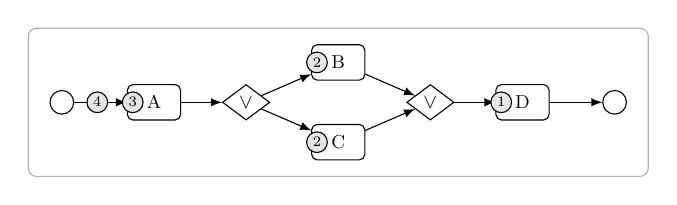
\begin{tikzpicture}[
    scale=0.75,
    every node/.style={transform shape},
    x=1.2cm, y=0.9cm, >=latex,
    event/.style={circle,draw,minimum size=4mm},
    gateway/.style={
        diamond,draw,
        aspect=2.4,
        minimum width=8mm,
        minimum height=6mm,
        inner sep=0pt,
        line width=0.4pt
    },
    activity/.style={rectangle,draw,rounded corners=2pt,
                     minimum width=9mm,minimum height=6mm,font=\small},
    case/.style={circle,draw,fill=black!10,
                 inner sep=0.5pt,minimum size=3.5mm,font=\scriptsize}
]

% nodes
\node[event]    (start) at (0,0) {};
\node[activity] (A)     at (1.3,0) {A};
\node[gateway]  (split) at (2.6,0) {};
\node[activity] (B)     at (3.9,0.75) {B};
\node[activity] (C)     at (3.9,-0.75) {C};
\node[gateway]  (join)  at (5.2,0) {};
\node[activity] (D)     at (6.5,0) {D};
\node[event]    (end)   at (7.8,0) {};

% OR symbols centered
\node at (split.center) {$\vee$};
\node at (join.center)  {$\vee$};

% arrows
\draw[->] (start) -- (A);
\draw[->] (A) -- (split);
\draw[->] (split) -- (B);
\draw[->] (split) -- (C);
\draw[->] (B) -- (join);
\draw[->] (C) -- (join);
\draw[->] (join) -- (D);
\draw[->] (D) -- (end);

% cases
\node[case] at (6.2, 0.00) {1};
\node[case] at (3.6, 0.75) {2};
\node[case] at (3.6,-0.75) {2};
\node[case] at (1.0, 0.00) {3};
\node[case] at (0.5, 0.00) {4};

% frame
\draw[gray!60, rounded corners=3pt]
  ($(current bounding box.south west)+(-0.3,-0.3)$)
  rectangle
  ($(current bounding box.north east)+(0.3,0.3)$);

\end{tikzpicture}
\caption{FIFO policy}
\label{fig:example-small-a}
\end{subfigure}
\hfill

% ===== Subfigure (b): Optimal =====
\begin{subfigure}{0.48\textwidth}
\centering
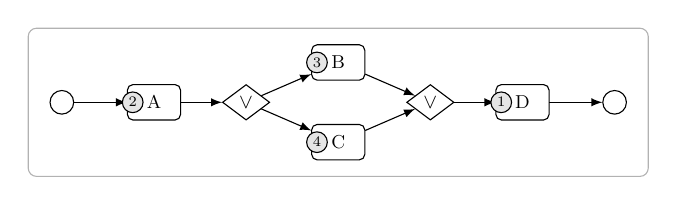
\begin{tikzpicture}[
    scale=0.75,
    every node/.style={transform shape},
    x=1.2cm, y=0.9cm, >=latex,
    event/.style={circle,draw,minimum size=4mm},
    gateway/.style={
        diamond,draw,
        aspect=2.4,
        minimum width=8mm,
        minimum height=6mm,
        inner sep=0pt,
        line width=0.4pt
    },
    activity/.style={rectangle,draw,rounded corners=2pt,
                     minimum width=9mm,minimum height=6mm,font=\small},
    case/.style={circle,draw,fill=black!10,
                 inner sep=0.5pt,minimum size=3.5mm,font=\scriptsize}
]

% nodes
\node[event]    (start) at (0,0) {};
\node[activity] (A)     at (1.3,0) {A};
\node[gateway]  (split) at (2.6,0) {};
\node[activity] (B)     at (3.9,0.75) {B};
\node[activity] (C)     at (3.9,-0.75) {C};
\node[gateway]  (join)  at (5.2,0) {};
\node[activity] (D)     at (6.5,0) {D};
\node[event]    (end)   at (7.8,0) {};

% OR symbols centered
\node at (split.center) {$\vee$};
\node at (join.center)  {$\vee$};

% arrows
\draw[->] (start) -- (A);
\draw[->] (A) -- (split);
\draw[->] (split) -- (B);
\draw[->] (split) -- (C);
\draw[->] (B) -- (join);
\draw[->] (C) -- (join);
\draw[->] (join) -- (D);
\draw[->] (D) -- (end);

% cases
\node[case] at (6.2, 0.00) {1};
\node[case] at (1.0, 0.00) {2};
\node[case] at (3.6, 0.75) {3};
\node[case] at (3.6,-0.75) {4};

% frame
\draw[gray!60, rounded corners=3pt]
  ($(current bounding box.south west)+(-0.3,-0.3)$)
  rectangle
  ($(current bounding box.north east)+(0.3,0.3)$);

\end{tikzpicture}
\caption{Case-aware optimal policy}
\label{fig:example-small-b}
\end{subfigure}

\caption{Comparison of completion times under (a) FIFO and (b) a case-aware optimal policy.}
\label{fig:example-small}
\end{figure}


\begin{example}\label{ex:intro}
Consider the workflow fragment in Figure~\ref{fig:example-small}, consisting of an activity $A$, an inclusive OR split into activities $B$ and $C$, an inclusive OR join, and a final activity $D$. Each activity utilizes a dedicated single server, and service times at $B$ and $C$ are both of unit length. Four cases exit $A$ in close succession, and the servers at $B$ and $C$ are initially idle.

The OR gate induces heterogeneous routing requirements. Cases 1 and 2 must complete both $B$ and $C$, while case 3 requires only $B$ and case 4 requires only $C$. A case completes once all of its required branches have finished.

Under a FIFO policy at $B$ and $C$ (Figure~\ref{fig:example-small-a}), cases are processed in arrival order at each activity. While this ordering is locally fair, it misaligns execution across branches. Cases that require synchronization are interleaved with cases that do not, causing avoidable waiting at the OR join. As a result, cases that traverse only a single branch complete later than necessary.


In contrast, a case-aware schedule aligns execution across branches (Figure~\ref{fig:example-small-b}), processing single-branch cases first and synchronized cases only
when all branches can progress, strictly reducing completion times.

Crucially, the failure of FIFO in this example cannot be repaired by tuning local priorities. It stems from the absence of a decision signal that reflects how current actions affect future synchronization.
\end{example} 

We propose to address the challenge of optimal dispatching where customers have varying time valuation by introducing a continuous \emph{value-of-time}
representation for cases.  
Each case reports a single temporal function describing
its marginal cost of waiting. This compact signal implicitly induces valuations over bundles of queue positions across all required activities, collapsing an exponential preference space into a tractable interface. Scheduling decisions that maximize aggregate reported value-of-time internalize delay externalities across queues, transforming scheduling at gateways into a structured strategic interaction between cases. Rather than viewing prioritization as inherently unfair, this perspective
interprets it as a mechanism for aligning individual incentives with global welfare in synchronization-constrained environments. We make the following three contributions:
\begin{enumerate}[label=(\arabic*),noitemsep,topsep=0pt,leftmargin=*]
\item We formalize a continuous value-of-time model for heterogeneous and time-varying waiting costs and define a welfare objective that generalizes weighted flow time.
\item We show how value-of-time functions encode bundle valuations across activities and how Vickrey--Clarke--Groves (VCG) style payments yield truthful reporting of value-of-time functions,
which serve as strategically sound primitives for creating
scheduling decisions in routed processes.
\item We develop a scheduling taxonomy for workflow fragments, characterizing XOR, AND, and OR fragments as distinct synchronization regimes, identifying when classical heuristics such as FIFO and SPT are structurally aligned or provably fail, and deriving locally and globally optimal scheduling rules for time-varying valuations.
\end{enumerate} The remainder of the paper is organized as follows. Section~\ref{sec:env} defines the problem setting. Section~\ref{sec:model} introduces the bidding model and its relation to the valuation view. Section~\ref{sec:scheduling} analyzes the induced scheduling regimes across XOR, AND, and OR gateways. Section~\ref{sec:exp} presents the empirical evaluation. Section~\ref{sec:related} reviews the related literature, and Section~\ref{sec:conclusion} concludes the paper.


% From an AI perspective, the proposed value-of-time layer can be viewed as a compact
% decision abstraction that transforms a high-dimensional, delayed, and
% synchronization-constrained scheduling problem into a sequential decision
% process with dense and interpretable rewards, enabling both mechanism-based
% optimization and learning-based control at the gateway level.







% \begin{example}\label{ex:intro}
% Consider the process presented in Figure~\ref{fig:example-small}. %$A \rightarrow$ OR split into $B$ and $C \rightarrow$ OR join $\rightarrow D \rightarrow$ end.
% Each of the four activities (marked A, B, C, and D) has a single server. Service times at $B$ and $C$ are unit length.
% Four cases leave $A$ at times $0,\tfrac{1}{4},\tfrac{1}{2},\tfrac{3}{4}$.
% The servers of $B$ and $C$ are idle at $t=0$.
% The gate in Figure~\ref{fig:example-small-b} is of type inclusive OR. Cases 1 and 2 must complete both $B$ and $C$ (similar to AND gate), case 3 needs only $B$, and case 4 needs only $C$ (similar to XOR gate).

% In what follows, we use $(s \rightarrow f)$ to denote the service interval of a case, from start time $s$ to completion time $f$ on the activity.

% Under FIFO policy (Figure~\ref{fig:example-small-a}), the schedule become %\ag{the meaning of the numbers in parantheses is unclear}
% \[
% \begin{array}{lcl}
% B: & \text{case 1 }(0\!\to\!1),\ \ \text{case 2 }(1\!\to\!2),\ \ \text{case 3 }(2\!\to\!3),\\[2pt]
% C: & \text{case 1 }(0\!\to\!1),\ \ \text{case 2 }(1\!\to\!2),\ \ \text{case 4 }(2\!\to\!3),
% \end{array}
% \]
% so the total completion time is
% \[
% \begin{array}{lcl}
% &T_{\text{c1}}=\max(1,1)=1,\quad
% T_{\text{c2}}=\max(2,2)=2,\\
% &T_{\text{c3}}=3,\quad
% T_{\text{c4}}=3,
% \end{array}
% \]
% and the mean $=[1+(2-1/4)+(3-1/2)+(3-3/4)]/4=1.875$.

% %\ag{why FIFO? isn't it optimal? should we call it optimal here or case-aware?} 
% An optimal ordering that aligns execution across branches (Figure~\ref{fig:example-small-b}) yields
% \[
% \begin{array}{lcl}
% B: & \text{case 1 }(0\!\to\!1),\ \text{case 3 }(1\!\to\!2),\ \text{case 2 }(2\!\to\!3),\\
% C: & \text{case 1 }(0\!\to\!1),\ \text{case 4 }(1\!\to\!2),\ \text{case 2 }(2\!\to\!3),
% \end{array}
% \]
% with completion times
% \[
% T_{\text{c1}}=1,\quad T_{\text{c2}}=3,\quad T_{\text{c3}}=2,\quad T_{\text{c4}}=2,
% \]
% and mean flow time $1.625$, a $13.3\%$ improvement. 
% \end{example}


% \section{Introduction}

% Service and workflow processes routinely involve queues in which cases incur heterogeneous and time-varying waiting costs~\citep{dumas2018fundamentals}. Nevertheless, common dispatching rules such as FIFO, static priorities, or shortest-processing-time (SPT) treat all cases as valuing time identically \citep{pinedo2012scheduling}. This assumption becomes especially problematic in business process networks containing XOR, AND, and inclusive OR gateways, where branching, concurrency, and synchronization create nonlinear dependencies between local scheduling decisions and global completion times \citep{senderovich2016conformance}.

% FIFO is often regarded as fair because it treats all cases symmetrically and avoids explicit prioritization \citep{hassin2003queue}. In contrast, value-based or priority-driven scheduling is frequently viewed as unfair, since it allows some cases to overtake others. This paper shows that this perceived tradeoff between fairness and efficiency is misleading. The conflict does not stem from prioritization itself, but from the absence of a mechanism that accounts for the delay externalities imposed by one case on another, a phenomenon well documented in strategic queueing models \citep{kleinrock1967optimum,lui1985equilibrium}. When waiting costs are represented explicitly and externalities are priced, prioritization can be both welfare-improving and procedurally fair.

% Business process control-flow models capture routing structures in which cases traverse activities and gateways \citep{dumas2018fundamentals}. An XOR gateway routes each case to exactly one branch, an AND gateway requires completion of all branches, and an OR gateway allows each case to require an arbitrary subset. OR gateways induce a partial concurrent open shop, in which cases must synchronize at a join after completing their selected branches \citep{pinedo2012scheduling,senderovich2016conformance}. In such settings, cases effectively value bundles of queue positions across multiple activities, and small local scheduling decisions can propagate into large global inefficiencies at synchronization points.

% \begin{example}
% %\ag{add a figure with the structure}  

% \begin{figure}[t!]
% \centering

% % ===== Subfigure (a): FIFO =====
% \begin{subfigure}{0.48\textwidth}
% \centering
% \begin{tikzpicture}[
%     scale=0.75,
%     every node/.style={transform shape},
%     x=1.2cm, y=0.9cm, >=latex,
%     event/.style={circle,draw,minimum size=4mm},
%     gateway/.style={
%         diamond,draw,
%         aspect=2.4,
%         minimum width=8mm,
%         minimum height=6mm,
%         inner sep=0pt,
%         line width=0.4pt
%     },
%     activity/.style={rectangle,draw,rounded corners=2pt,
%                      minimum width=9mm,minimum height=6mm,font=\small},
%     case/.style={circle,draw,fill=black!10,
%                  inner sep=0.5pt,minimum size=3.5mm,font=\scriptsize}
% ]

% % nodes
% \node[event]    (start) at (0,0) {};
% \node[activity] (A)     at (1.3,0) {A};
% \node[gateway]  (split) at (2.6,0) {};
% \node[activity] (B)     at (3.9,0.75) {B};
% \node[activity] (C)     at (3.9,-0.75) {C};
% \node[gateway]  (join)  at (5.2,0) {};
% \node[activity] (D)     at (6.5,0) {D};
% \node[event]    (end)   at (7.8,0) {};

% % OR symbols centered
% \node at (split.center) {$\vee$};
% \node at (join.center)  {$\vee$};

% % arrows
% \draw[->] (start) -- (A);
% \draw[->] (A) -- (split);
% \draw[->] (split) -- (B);
% \draw[->] (split) -- (C);
% \draw[->] (B) -- (join);
% \draw[->] (C) -- (join);
% \draw[->] (join) -- (D);
% \draw[->] (D) -- (end);

% % cases
% \node[case] at (6.2, 0.00) {1};
% \node[case] at (3.6, 0.75) {2};
% \node[case] at (3.6,-0.75) {2};
% \node[case] at (1.0, 0.00) {3};
% \node[case] at (0.5, 0.00) {4};

% % frame
% \draw[gray!60, rounded corners=3pt]
%   ($(current bounding box.south west)+(-0.3,-0.3)$)
%   rectangle
%   ($(current bounding box.north east)+(0.3,0.3)$);

% \end{tikzpicture}
% \caption{FIFO policy}
% \label{fig:example-small-a}
% \end{subfigure}
% \hfill

% % ===== Subfigure (b): Optimal =====
% \begin{subfigure}{0.48\textwidth}
% \centering
% \begin{tikzpicture}[
%     scale=0.75,
%     every node/.style={transform shape},
%     x=1.2cm, y=0.9cm, >=latex,
%     event/.style={circle,draw,minimum size=4mm},
%     gateway/.style={
%         diamond,draw,
%         aspect=2.4,
%         minimum width=8mm,
%         minimum height=6mm,
%         inner sep=0pt,
%         line width=0.4pt
%     },
%     activity/.style={rectangle,draw,rounded corners=2pt,
%                      minimum width=9mm,minimum height=6mm,font=\small},
%     case/.style={circle,draw,fill=black!10,
%                  inner sep=0.5pt,minimum size=3.5mm,font=\scriptsize}
% ]

% % nodes
% \node[event]    (start) at (0,0) {};
% \node[activity] (A)     at (1.3,0) {A};
% \node[gateway]  (split) at (2.6,0) {};
% \node[activity] (B)     at (3.9,0.75) {B};
% \node[activity] (C)     at (3.9,-0.75) {C};
% \node[gateway]  (join)  at (5.2,0) {};
% \node[activity] (D)     at (6.5,0) {D};
% \node[event]    (end)   at (7.8,0) {};

% % OR symbols centered
% \node at (split.center) {$\vee$};
% \node at (join.center)  {$\vee$};

% % arrows
% \draw[->] (start) -- (A);
% \draw[->] (A) -- (split);
% \draw[->] (split) -- (B);
% \draw[->] (split) -- (C);
% \draw[->] (B) -- (join);
% \draw[->] (C) -- (join);
% \draw[->] (join) -- (D);
% \draw[->] (D) -- (end);

% % cases
% \node[case] at (6.2, 0.00) {1};
% \node[case] at (1.0, 0.00) {2};
% \node[case] at (3.6, 0.75) {3};
% \node[case] at (3.6,-0.75) {4};

% % frame
% \draw[gray!60, rounded corners=3pt]
%   ($(current bounding box.south west)+(-0.3,-0.3)$)
%   rectangle
%   ($(current bounding box.north east)+(0.3,0.3)$);

% \end{tikzpicture}
% \caption{Optimal policy}
% \label{fig:example-small-b}
% \end{subfigure}

% \caption{Comparison of FIFO (a) to the optimal policy (b).}
% \label{fig:example-small}
% \end{figure}

% Consider $A \rightarrow$ OR split into $B$ and $C \rightarrow$ OR join $\rightarrow D \rightarrow$ end.
% Each activity has a single server. Service times at $B$ and $C$ are identically distributed with unit length in expectation.
% Four cases leave $A$ at times $0,\tfrac{1}{4},\tfrac{1}{2},\tfrac{3}{4}$.
% The servers of $B$ and $C$ are idle at $t=0$.
% Requirements: cases 1 and 2 must complete both $B$ and $C$ (AND). case 3 needs only $B$ and case 4 needs only $C$.

% Under FIFO policy, the schedule become
% \[
% \begin{array}{lcl}
% B: & \text{case 1 }(0\!\to\!1),\ \ \text{case 2 }(1\!\to\!2),\ \ \text{case 3 }(2\!\to\!3),\\[2pt]
% C: & \text{case 1 }(0\!\to\!1),\ \ \text{case 2 }(1\!\to\!2),\ \ \text{case 4 }(2\!\to\!3),
% \end{array}
% \]
% so the total completion time is
% \[
% \begin{array}{lcl}
% &T_{\text{c1}}=\max(1,1)=1,\quad
% T_{\text{c2}}=\max(2,2)=2,\\
% &T_{\text{c3}}=3,\quad
% T_{\text{c4}}=3,
% \end{array}
% \]
% and the mean $=[1+(2-1/4)+(3-1/2)+(3-3/4)]/4=1.875$.

% With case-aware selection, a feasible ordering is
% \[
% \begin{array}{lcl}
% B: & \text{case 1 }(0\!\to\!1),\ \ \text{case 3 }(1\!\to\!2),\ \ \text{case 2 }(2\!\to\!3),\\[2pt]
% C: & \text{case 1 }(0\!\to\!1),\ \ \text{case 4 }(1\!\to\!2),\ \ \text{case 2 }(2\!\to\!3),
% \end{array}
% \]
% which yields
% \[
% \begin{array}{lcl}
% &T_{\text{c1}}=\max(1,1)=1,\quad
% T_{\text{c2}}=\max(3,3)=3,\\
% &T_{\text{c3}}=2,\quad
% T_{\text{c4}}=2,
% \end{array}
% \]
% and the mean $=[1+(3-1/4)+(2-1/2)+(2-3/4)]/4=1.625$, about an $13.3\%$ improvement. SPT does not help here since $B$ and $C$ have equal/unknown durations. The gain in this case is aligning branch.

% \end{example}

% The running example illustrates a structural limitation of treating queues independently. FIFO appears locally fair at each activity, yet it produces avoidable global delay once synchronization is taken into account. The inefficiency does not arise from strategic manipulation, but from the fact that FIFO fails to account for how advancing a case on one branch affects the join time of others. Similar misalignments are known to arise in open shop and synchronization-constrained scheduling settings \citep{pinedo2012scheduling}.

% We address this challenge by introducing a continuous \emph{value-of-time} representation. Instead of bidding on discrete queue positions or combinatorial allocations, each case reports a single temporal function describing its marginal cost of delay. This function implicitly defines valuations over admissible bundles of queue positions across required branches. When scheduling decisions maximize aggregate reported value-of-time and Vickrey--Clarke--Groves (VCG) payments are applied, FIFO emerges as the zero-externality baseline, while deviations are governed by payments that exactly price the delay imposed on others, consistent with classic results in priority pricing and mechanism design \citep{mendelson1990priority,nisan2007algorithmic}. As a result, truthful reporting aligns individual incentives, social welfare, and fairness.

% Building on this representation, we develop a unified taxonomy of gateway-level scheduling regimes. We characterize when XOR, AND, and OR gateways admit structurally aligned local scheduling rules and when classical heuristics such as FIFO and SPT fail due to synchronization effects. For gateway cases that are analytically intractable, including general OR-routing fragments, we complement our theoretical analysis with an empirical evaluation that quantifies the welfare gains of valuation-driven scheduling. Finally, we show that the same valuation layer induces a dynamic local scheduling rule that generalizes classical $c\mu$ and Smith ratio rules to time-varying valuations, and that it provides a dense and interpretable reward signal for reinforcement learning.

% \paragraph{Contributions.}
% This paper makes the following contributions:
% \begin{itemize}
% \item We introduce a continuous value-of-time representation for expressing heterogeneous and time-varying waiting costs in business processes and define a welfare objective that generalizes weighted flow time.
% \item We show how value-of-time functions implicitly encode valuations over bundles of queue positions and how VCG-style payments reconcile efficiency and fairness by pricing delay externalities.
% \item We develop a scheduling-theoretic taxonomy of BPM gateways, characterizing XOR, AND, and OR fragments as distinct scheduling regimes and identifying when classical heuristics are structurally adequate.
% \item We derive dynamic local scheduling rules for time-varying valuations and demonstrate how the same valuation layer supports empirical evaluation.
% \end{itemize}


% \section{Introduction}
% \ag{revise structure to the following paragraphs: 1. Introduction of the environment (the current text is good). 2. Introduction of the problem (don't dwell into related work), 3. Our solution, 4. Our contribution, 5. Structure of the rest of the paper}

% Service and workflow processes routinely involve queues in which cases incur highly heterogeneous waiting costs. Nevertheless, common dispatching rules such as FIFO, static priorities, or shortest-processing-time (SPT) treat all cases as valuing time identically. This assumption becomes especially problematic in Business Process Management (BPM) networks containing XOR, AND, and particularly OR gateways, where branching, concurrency, and synchronization create nonlinear dependencies between local scheduling decisions and global completion times.

% BPM control-flow models \citep{dumas2018fundamentals} capture routing structures, where OR-gateways are common. Such gateways induce a \emph{partial concurrent open shop} (PCOS), in which cases require arbitrary subsets of activities and must later synchronize at a join \citep{pinedo2012scheduling,senderovich2016conformance}. Completion times are determined by the maximum over multiple branches, and each case effectively values \emph{bundles of queue positions} across several activities. The following example illustrates the structural inefficiency of treating queues independently in such settings.



% Despite the centrality of OR-gateways in real processes, current scheduling frameworks lack a compact way to express how cases value joint completion across multiple branches. Traditional single-queue prioritization rules (e.g., \cite{Pinedo2016,HarcholBalter2013}) fail to capture synchronization effects, while strategy-oriented models for priority bidding (e.g., \cite{Kleinrock1967,MendelsonWhiting2018}) address only isolated queues and do not extend to multi-branch completion. As a result, even conceptually simple routed processes lack an appropriate representation for heterogeneous waiting costs.

% We address this challenge by introducing a continuous \emph{value-of-time} representation: instead of bidding on discrete allocations or queue positions, each case reports a marginal waiting-cost function over time. This single temporal signal implicitly induces valuations over bundles of positions across all required branches, enabling VCG-style reasoning at gateways without explicit combinatorial bidding. Conceptually, it collapses an exponential valuation space into a tractable, strategic, and process-compatible interface.

% Building on this idea, this paper makes four contributions.  
% \textbf{(1)} We introduce a continuous value-of-time representation for case preferences and define a welfare objective generalizing weighted flow-time.  
% \textbf{(2)} We show how value-of-time functions implicitly encode bundle valuations and how VCG-style payments yield truthful reporting in structured workflow settings.  
% \textbf{(3)} We develop the first scheduling-theoretic taxonomy that characterizes workflow gateways (XOR, AND, and OR) as distinct scheduling regimes, identifying when FIFO aligns with synchronization and when it fails.  
% \textbf{(4)} We prove that value-of-time reporting induces a dynamic local scheduling rule that generalizes classical $c\mu$ and Smith’s ratio rules to time-varying valuations, and we demonstrate how the same valuation layer provides a dense, interpretable reward signal for reinforcement learning agents.

%Overall, this framework bridges BPM, scheduling theory, mechanism design, and reinforcement learning by replacing ad-hoc priorities and infeasible combinatorial auctions with a compact, strategic, and learning-compatible interface for case-aware decision-making in routed processes.

%The remainder of the paper is organized as follows.  
%Section "Model" formalizes the BPM routing and valuation model and develops the induced bundle valuations and VCG-style payment rule.  
%Section "Scheduling" derives the resulting dynamic scheduling policy.  
%Section "RL" demonstrates how the valuation layer enables dense RL rewards and improves learning stability.  
%Section "Experiments" presents simulation results, and Section "Conclusion" concludes.














% =====================================
\section{Problem Setting}
\label{sec:env}

% =====================================

In this section, we formulate the scheduling problem studied in this paper. 
We begin by defining a workflow fragment, a process building block that a case encounters during execution. 
We then define gateway semantics and formalize resource and service dynamics, the resulting decision epochs, and the case-selection problem faced by the scheduler, allowing cases to incur heterogeneous and time-dependent costs of delay.

\subsection{Workflow Fragments}

We consider a {\em workflow fragment}
to be a part of a workflow network that consists of a single split gateway 
that branches into multiple activities and later
synchronizes at a corresponding join.
\begin{definition}\label{def:processFragment}
A {\em workflow fragment} is a sextuple $\mathcal{P} = (A, g, \mathrm{Succ}(g), T, R, \lambda)$
where:
\begin{itemize}
  \item $A$ is a set of activities.
  \item $g$ is a split gateway with successors
        $\mathrm{Succ}(g)=\{a_1,\dots,a_m\}\subseteq A$.
  \item $T \subseteq (A \cup \{g\}) \times (A \cup \{g\})$ is the
        control-flow relation.
  \item $R$ is a set of resources, each capable of processing at
        most one case at a time.
  \item $\lambda : A \to 2^R$ maps each activity to the resources that
        can execute it. 
\end{itemize}
\end{definition} \noindent Cases arrive over time and
traverse the fragment according to the control-flow induced by the
gateway. Specifically, case $i$ requires a non-empty subset
$S_i \subseteq \{1,\dots,m\}$ of activities it must complete prior to leaving
the fragment. This induces the following standard gateway
semantics for $g$ ~\citep{dumas2018fundamentals}:
\begin{itemize}
  \item \textbf{XOR:} $|S_i|=1$.  The case selects exactly one branch.
  \item \textbf{AND:} $S_i = \{1,\dots,m\}$.  The case must complete all the activities before the join.
  \item \textbf{OR:} $S_i$ is an arbitrary non-empty subset.  The case
        requires a bundle of activities, yielding a partial concurrent
        open shop structure.
\end{itemize}

%



%\ag{demonstrate using Example~\ref{ex:intro}}


Let $C_{i,a}$ denote the completion time of case $i$ on activity $a$.
Its completion time at the join is $C_i \;=\; \max_{a \in S_i} C_{i,a}$, reflecting synchronization on the slowest branch.\footnote{Activity $a_i$ may represent abstract sub-processes that contain
a drill-down to additional activities and gateways. 
In this paper, we consider $a_i$ to be `black-box' tasks
without going into an interpretation of sub-process vs. activity.}



\setcounter{example}{0}
\begin{example}[cont]
The gateway in Figure~\ref{fig:example-small} is an OR-gateway.
Cases 1 and 2 require both activity $b$ and $c$, while case 3 requires only activity $B$ and case 4 requires only activity $C$.
Each case completes the fragment only after synchronizing all required activities.
\end{example}

\subsection{Resources and Service Dynamics}

Each activity $a$ is assigned a set of resources $\lambda(a)$ and each resource
processes the cases in a queueing order.  
For ease of presentation, we assume that 
each activity $a$ is served by a single resource ($\lambda(a) = r_a \in R$). This simplifying assumption allows us to focus on the complementary 
problem of allocating cases to activities.

Time is continuous, but service completions, case arrivals, and
resource releases give rise to a discrete event sequence
$\mathcal{E} = \{\tau_1 < \tau_2 < \dots\}$.  
Scheduling and allocation decisions occur only at these decision
epochs.

We assume deterministic service times that may vary across
cases even at the same activity.  
At any event $\tau$, each activity $a$ has a queue of waiting cases.  We assume non-preemptive services. Therefore, once service of a case begins, it must be completed without interruption.
Once all required activities are completed, there is a join operation that allows 
the case to exit the fragment.

\subsection{Decision Problem}

At each decision epoch $\tau$, whenever the dedicated resource of
activity $a$ becomes idle, the scheduler must select a case from $a$'s
queue.  Formally, the decision at time $\tau\in\mathcal{E}$ is a mapping
$d_\tau : A^{\mathrm{ready}}(\tau) \to \mathcal{I} \cup \{\bot\}$,
where $A^{\mathrm{ready}}(\tau)$ is the set of activities whose
resource is idle, $\mathcal{I}$ is the set of active cases,
and $\bot$ indicates that the activity remains idle.


The central problem studied in this work is \emph{case selection}: given the current queues and the partial progress of all cases, \emph{which case should an available resource start next at a given activity so as to minimize a social objective that accounts for heterogeneous waiting costs and synchronization at the join?}

%\subsection{Case Types and Routing Semantics}

\subsection{Value-of-Time Function}

Each case $i$ is assumed to have an inherent piecewise-continuous \emph{value-of-time} function
$v_i(t)\ge 0$ that specifies its instantaneous marginal cost of
remaining in the process at time $t$. This representation is strictly
more expressive than fixed priorities or static weights. It allows the
urgency of a case to evolve over time and to depend on business
constraints, deadlines, or commitments.

Different shapes correspond to different operational semantics:
 On the one hand, a high, nearly constant $v_i(t)$ models high-priority
  cases, such as VIP customers, urgent financial applications, or
  high-acuity patients in healthcare triage.
  On the other hand, a low or slowly varying $v_i(t)$ represents cases that are
 insensitive to delay, such as routine customer requests or
  non-urgent diagnostic procedures.
 Finally, an interesting special case is a function that increases sharply near a deadline, captures cases facing contractual penalties, SLAs, or clinical thresholds where
  delay rapidly escalates risk.
% By allowing $v_i(t)$ to vary over time, this representation subsumes
% static priorities and weighted flow-time models while modeling
% time-dependent and case-specific urgency profiles.

\subsection{Scheduling Objectives}
Given a realization of the schedule, let $I_\mathcal{P}(t)$ denotes the set of cases present in the fragment at time $t$. The total waiting
cost of case $i$ is given by,
\begin{equation}
\label{eq:case_welfare}
W_i \;=\; \int_0^\infty v_i(t)\,\mathbf{1}\!\left\{ i \in I_{\mathcal{P}}(t) \right\}\, dt
\end{equation}


A natural social objective is to minimize the long-run average
aggregate value-of-time in the system:
\begin{equation}
\label{eq:infinte_welfare}
W_\infty = \lim_{T \to \infty} \frac{1}{T} \int_0^T
\sum_{i \in I_\mathcal{P}(t)} v_i(t)\, dt
\end{equation}

In finite-horizon or offline settings, we can equivalently minimize
$\sum_i W_i$, which generalizes both unweighted and weighted flow-time
objectives \citep{schrage1968sequencing}.


% =====================================
\section{Bidding for Workflow Fragments}
\label{sec:model}

% =====================================
% While our setting specifies how delays arise and how XOR, AND, and OR
% semantics shape completion times, it leaves open how cases should
% express their preferences over these delay profiles. A direct bidding
% approach would require cases to report valuations over combinatorial
% bundles of queue positions creating an intractable space even in simple OR
% fragments. This motivates our shift to continuous value-of-time
% functions, which compactly encode all relevant bundle valuations and
% allow us to analyze the structural scheduling regimes captured in our
% taxonomy.

%\subsection{Naive Bidding and Combinatorial Explosion}
% When
% reaching a process fragment (a decision point in a workflow), 
% cases compete for execution capacity.
% The system can be described from two points of view: a \emph{valuation} view, in which each case is characterized by a value-of-time function, and a \emph{bidding} view, in which cases express these valuations through bids.
% However, in the presence of 
% routing and synchronization, case utility depends jointly on the execution of multiple concurrent 
% activities, as shown in Example~\ref{ex:intro}.

% In order to optimize equation ~\eqref{eq:infinte_welfare}, we need approach to the value of time function of each case. truthful.
% To do so, we define a truthful bidding mechanism based on the reported \emph{value-of-time} functions. 

% Below, we resolve the competition by defining 
% a bidding mechanism based on value-of-time functions.
% Specifically, cases will submit ... and then ... and lastly,...
% To address this challenge, we define a bidding mechanism based on
% \emph{value-of-time} functions.
To optimize Equation~\eqref{eq:infinte_welfare}, 
one must obtain a value-of-time function of the case.
However, the true functions are not explicitly known,
and must be elicited from the cases. 
To this end, we design a bidding mechanism in which cases report value-of-time functions and truthfulness follows by construction.

Formally, a \emph{bundle} $B$ is a finite set of $(a,k)$ pairs, where $a$ denotes an activity
of the workflow fragment and
$k \in \mathbb[n(a)]$ denotes a position in the local execution order of activity $a$, where $n(a)$ is the number of cases in 
 queue for $a$. A bundle $B$ is \emph{admissible} if the following conditions hold:
\begin{enumerate}
    \item \emph{No duplication per activity}.  
    If $(a,\cdot)\in B$ and $(a,\cdot)'\in B$, they refer to the same item.
   \item \emph{Gateway consistency:} the set of activities appearing in $B$ is consistent with the gateway semantics defined for the process.
\end{enumerate}  When considering multiple cases simultaneously, we require that no two cases are assigned the same pair $(a,k)$. At most one case may occupy each position.
\begin{definition}[Bid function]
Let $\mathcal{B}_i(\mathcal{P},\tau)$ be the set of all \emph{admissible bundles} for case $i$. A \emph{bid function} $b_i$ for case $i$ is a full mapping: \[
    b_i:\mathcal{B}_i(\mathcal{P},\tau) \rightarrow \mathbb{R},
\]
that gives a valuation to each admissible bundle $B$ for case $i$ at time $\tau$. 
\end{definition}  
While conceptually natural, the proposed bidding mechanism is infeasible,
since the number of admissible bundles grows
exponentially in the number of outgoing branches \citep{sandholm2002algorithm}, and each case must report valuations over the entire state-space.
Moreover, winner determination requires solving a combinatorial
allocation problem at each decision epoch $\tau\in\mathcal{E}$.
 
To overcome this combinatorial explosion, we reposition the problem
from bidding for all possible bundles to reporting 
a single value-of-time function which generalizes the bidding mechanism, 
and remains tractable for most cases
that we consider in this paper.


As a first step, fix a workflow fragment $\mathcal{P}$ at time $\tau$.
Each case $i\in\mathcal{I}_\mathcal{P}(\tau)$ submits $\hat v_i(t)$.
Let $\pi^{\mathrm{H}}$ be a baseline policy
(e.g., FIFO or any other heuristic) computed from the observed state, inducing join time $\tau_i^{\mathrm{H}}$ for case $i$.
For an admissible bundle $B$ of case $i$, let $\tau_i^{\hat v}(B)$ denote the
join time that case $i$ can achieve under the optimal policy (minimizing Eq.~\eqref{eq:infinte_welfare})
that is consistent with $B$.


Next, we define $b_i(B)$ as 
\begin{equation} \label{eq:bidding}
\quad b_i(B)\ :=\ \int_{\tau_i^{\hat v}(B)}^{\ \ \tau_i^{\mathrm{H}}}\! \hat v_i(u)\,du.\quad
\end{equation} 
This expression is the waiting-cost \emph{reduction}
relative to the baseline and may be negative when $\tau_i^{\hat v}(B)>\tau_i^{\mathrm{H}}$, i.e., case  
$i$ may worsen compared to $\pi^{\mathrm{H}}$. In the negative case, instead of paying for a bundle, 
the case receives a compensation at that is at
least equivalent to what the case lost compared to the heuristic policy. 
This induces an implicit game among the cases.\footnote{The relationship between
bidding and game theory was established in~\citep{lui1985bribery}.}

One may define a policy fairness criterion relative to FIFO, which serves as a widely used heuristic and a neutral, allocation-independent baseline. Let $\tau_i^{FIFO}$ denote the completion time of case $i$ under FIFO. A positive value of Eq.~\eqref{eq:bidding} corresponds to an \emph{entitled overtake}, in which case $i$ overtakes other cases, while a negative value indicates that case $i$ is overtaken by others. Deviations from FIFO arise only when justified by heterogeneous urgency and are regulated through value-of-time payments that price the induced delay imposed on other cases.
% preserving both efficiency and truthful reporting.  

\begin{theorem}
Maximizing the sum of bids, $\sum_i b_i(B)$, is equivalent to minimizing 
the finite-horizon social objective, namely $\sum_i W_i$.
\end{theorem}
\begin{proof}
Since $\tau_i^{\mathrm{H}}$ is auction-independent,
\begin{equation}
\begin{aligned}
\sum_i b_i(B)
&= \sum_i\int_{\tau^{\hat v_i(B)}}^{\tau_i^{\mathrm{H}}} \hat v_i(u)\,du \\[0.8em]
&= \sum_i\Big(
   \underbrace{\int_{t}^{\tau_i^{\mathrm{H}}} \hat v_i(u)\,du}_{\text{constant}}
   - \int_{t}^{\tau^{\hat v_i(B)}}\hat  v_i(u)\,du
   \Big).
\end{aligned}
\end{equation}
Therefore, maximizing $\sum_i b_i(B)$ is equivalent to minimizing $\sum_i W_i$.
\end{proof}


\ifconf
In the technical appendix, we show how payments constructed from the bids
in Eq.~\eqref{eq:bidding} are aligned with VCG-style externality pricing.
This establishes that truthful reporting of the value-of-time function is a
dominant strategy within the expressive reporting model, allowing reported
valuations to be treated as truthful primitives for analysis
\citep{groves1973,clarke1971,vickrey1961}.
Importantly, this incentive result is conceptual rather than algorithmic:
it does not imply that welfare-maximizing allocations are computationally
tractable in all routing regimes.
Rather, it justifies replacing intractable combinatorial bundle bidding with
a compact and strategically sound functional representation, which in turn
enables structural characterization and tractable analysis in several
important scheduling regimes.
Non-participation is modeled by reporting $v_i(t)\equiv 0$, which schedules
the case last and ensures individual rationality (see technical appendix).


\else
\begin{lemma}[Truthful bidding is a dominant strategy in Stage~2]\label{lem:truthful}
Let $\mathcal{B}_i(g,\tau)$ be the set of admissible bundles with reported bids
$b_i:\mathcal{B}_i(g,\tau)\to\mathbb{R}_{\ge0}$. The model selects an allocation
\[
x^\star(b)\in\arg\max_{x}\ \sum_{j\in I_g(\tau)}\sum_{B\in\mathcal{B}_j(g,\tau)} b_j(B)\,x_{j,B}
\]
and payments
\[
p_i\ :=\ W_{-i}\;-\!\!\sum_{j\neq i}\sum_{B\in\mathcal{B}_j(g,\tau)} b_j(B)\,x^\star_{j,B}(b),
\quad
\]
\[
W_{-i}\ :=\ \max_{x}\ \sum_{j\neq i}\sum_{B} b_j(B)\,x_{j,B}.
\]
Let $v_i:\mathcal{B}_i(g,\tau)\to\mathbb{R}_{\ge0}$ be $i$'s true valuation on bundles.
Then the truthful report $b_i=v_i$ is a dominant strategy for case $i$.
\end{lemma}

\begin{proof}[Proof]
Fix a bid-profile of functions $(\hat b_i(\cdot),\, b_{-i}(\cdot))$, where
$\hat b_i:\mathcal{B}_i(g,\tau)\!\to\!\mathbb{R}_{\ge0}$ and
for each $j\neq i$, $b_j:\mathcal{B}_j(g,\tau)\!\to\!\mathbb{R}_{\ge0}$.
Let $x^\star=x^\star(\hat b_i(\cdot),b_{-i}(\cdot))$ be a WDP maximizer in Stage~2.
By definition,
\[
p_i \;=\; W_{-i}\;-\!\!\sum_{j\neq i}\sum_{B\in\mathcal{B}_j(g,\tau)} b_j(B)\,x^\star_{j,B}(\hat b_i(\cdot),b_{-i}(\cdot)),
\]
where $W_{-i}=\max_{x}\sum_{j\neq i}\sum_{B} b_j(B)\,x_{j,B}$ depends only on $b_{-i}(\cdot)$.

The utility of $i$ under its true valuation function $v_i:\mathcal{B}_i(g,\tau)\!\to\!\mathbb{R}_{\ge0}$ is

\begin{align*}
u_i(\hat b_i(\cdot),b_{-i}(\cdot);v_i)
&= \sum_{B} v_i(B)\,
   x^\star_{i,B}(\hat b_i(\cdot),b_{-i}(\cdot)) - p_i\\
&= \sum_{B} v_i(B)\,
   x^\star_{i,B}(\hat b_i(\cdot),b_{-i}(\cdot))\\
&\quad+ \sum_{j\neq i}\sum_{B} b_j(B)\,
   x^\star_{j,B}(\hat b_i(\cdot),b_{-i}(\cdot))
   - W_{-i}\\
&= \sum_{j}\sum_{B} w_j(B)\,
   x^\star_{j,B}(\hat b_i(\cdot),b_{-i}(\cdot)) - W_{-i}.
\end{align*}

where we set $w_i:=v_i$ and $w_j:=b_j$ for all $j\neq i$.

Since $W_{-i}$ is independent of $\hat b_i(\cdot)$, maximizing $u_i$ over the entire function $\hat b_i(\cdot)$
is equivalent to maximize $\sum_{j,B} w_j(B)\,x_{j,B}$.
But Stage~2 selects
\[
x^\star(\hat b_i(\cdot),b_{-i}(\cdot))\in\arg\max_{x}\ \sum_{j}\sum_{B} \tilde b_j(B)\,x_{j,B},
\quad
\]
\[
\text{with }\ \tilde b_i=\hat b_i,\ \tilde b_j=b_j\ (j\neq i).
\]
For the mechanism to choose the allocation that is best
according to your \emph{true} preferences, it must maximize a sum in which
your contribution equals your true value for \emph{each} bundle. But the
mechanism maximizes the \emph{reported} sum. Therefore, the only way to make
the reported objective coincide with the true one is to report your value
\emph{truthfully for every bundle}.
Consequently, truthful bidding is weakly dominates any alternative report.
\qedhere
\end{proof}



\begin{lemma}[The bidding mechanism is individually rational]\label{lem:IR-bids}
In the setting of Lemma~\ref{lem:truthful}, With payments $p_i(b)$ as above, the truthful utility is nonnegative using the strategy of reporting $v_i(B)$ for all $B\in\mathcal{B}_i(g,\tau)$:
\[
u_i(v_i,b_{-i};v_i)\ =\ \sum_{B} v_i(B)\,x^\star_{i,B}(v_i,b_{-i})\ -\ p_i(v_i,b_{-i})\ \ge\ 0.
\]
\end{lemma}

\begin{proof}[Proof]
Define
\[
W(v_i,b_{-i})\ :=\ \max_{x}\Bigg\{\sum_{B} v_i(B)\,x_{i,B}\;+\!\!\sum_{j\neq i}\sum_{B} b_j(B)\,x_{j,B}\Bigg\}.
\]
In the technical appendix we show how we build payments from the bids based on a baseline policy and proof that they are aliened with VCG payments, $u_i(v_i,b_{-i};v_i)=W(v_i,b_{-i})-W_{-i}(b_{-i})$.
Because the feasible set with $i$ present contains every allocation that simply ignores $i$,
$W(v_i,b_{-i})\ge \max_x \sum_{j\neq i}\sum_B b_j(B)\,x_{j,B}=W_{-i}(b_{-i})$.
Thus $u_i\ge 0$.\qedhere
\end{proof}
\fi
 

%Moreover, when the social planner implements a welfare-maximizing schedule
%based on the reported
%$v_i(t)$, a VCG mechanism at gateways can make truthful reporting a
%dominant strategy. 











%\subsection{Strategic Properties}





% =====================================


\section{Scheduling in Workflow Fragments}
\label{sec:scheduling}


We identify six scheduling regimes 
in a workflow fragment $\mathcal{P}$ with $m$ parallel
activities that arise from different
combinations of two degrees of freedom:
\textbf{(1)} gateway semantics (XOR/AND/OR) and, 
\textbf{(2)} valuation structure (constant or time-varying).
Processing times $p_{i,a}$ are allowed to be heterogeneous across cases and activities.

Note that an XOR gateway can equivalently be modeled as a choice among $m$
single-activity branches. Consequently, the taxonomy implicitly abstracts
away a third degree of freedom, namely whether the gateway consists of a
single activity or of $m$ parallel activities. 

The taxonomy, presented in Table~\ref{tab:taxonomy}, is complete within our modeling assumptions and highlights how essential the partition into cases can be.
Due to space consideration, we provide detailed descriptions of Cases 2 and 3 for which we obtained theoretical results.
Our experiments will cover additional cases (Cases 4 and 6) for which tractability was not established. 

%complete and highlights how essential case-aware selection is.
%\subsection{A Taxonomy of Gateway-Level Cases}
%\label{sec:taxonomy}

% \begin{figure}[t]
% \centering
% \begin{tikzpicture}[x=1.2cm,y=0.9cm]

%   % start / split / join / end
%   \node[event]   (start) at (0,0) {};
%   \node[gateway] (split) at (1.2,0) {};
%   \node[gateway] (join)  at (5.0,0) {};
%   \node[event]   (end)   at (6.2,0) {};

%   % OR marks
%   \node at (split) {$\vee$};
%   \node at (join)  {$\vee$};

%   % activities
%   \node[activity] (a1) at (3.0,  1.0) {$a_1$};
%   \node[activity] (a2) at (3.0,  0.0) {$a_2$};
%   \node           (dots) at (3.0, -0.8) {$\vdots$};
%   \node[activity] (am) at (3.0, -1.6) {$a_m$};

 
%   \begin{scope}[on background layer]
%     \node[fragment, rectangle, fit=(split) (a1) (a2) (am) (join), inner sep=6mm] (frame) {};
%   \end{scope}

%   % main solid flows
%   \draw[flow] (start) -- (split);
%   \draw[flow] (split) -- (a1.west);
%   \draw[flow] (split) -- (a2.west);
%   \draw[flow] (split) -- (am.west);

%   \draw[flow] (a1.east) -- (join);
%   \draw[flow] (a2.east) -- (join);
%   \draw[flow] (am.east) -- (join);
%   \draw[flow] (join) -- (end);

%   % dashed subset flows
%   \draw[dashedflow] (split.south) .. controls (1.4,-1.3) and (2.2,-1.3) .. (a1.west);
%   \draw[dashedflow] (split.south) .. controls (1.6,-1.5) and (2.2,-1.5) .. (a2.west);
%   \draw[dashedflow] (split.south) .. controls (1.8,-2.0) and (2.2,-2.0) .. (am.west);

% \end{tikzpicture}
% \caption{OR-routing fragment forming a partial concurrent open shop (PCOS):
% each case selects a subset $S_i$ of branches and must synchronize at the join.}
% \label{fig:or-pcos}
% \end{figure}


\begin{table*}[t!]
\centering
\small
\setlength{\tabcolsep}{1pt}  
\begin{tabular}{|c|p{4.9cm}|p{4.9cm}|p{4.9cm}|}
\hline
\textbf{Valuation} 
& \textbf{XOR} 
& \textbf{AND} 
& \textbf{OR} \\
\hline
\textbf{Constant $v_i(t)=v_i$}
&
Case 1: Reduces to a single-server queue with heterogeneous constant weights.
The induced objective is weighted flow-time minimization.
\emph{WSPT} is optimal~\citep{smith1956various}.
If all $v_i$ are identical, \emph{SPT} is optimal~\citep{schrage1968sequencing}.
&
Case 3: Synchronization (permutation consistent across activities) is required to prevent inefficiency when processing times differ across activities.
Any inverted schedule is weakly dominated (Lemma~\ref{lem:inv-dominated}), explaining why FIFO is structurally aligned.
Experimental results support this claim.
&
Case 5: 
Even with constant and identical valuations, heterogeneous routing together with activity-dependent processing times induce asymmetric synchronization.
Per-branch FIFO or WSPT rules are structurally misaligned and may increase join delay.

\\
\hline
\textbf{Time-varying $v_i(t)$}
&
Case 2: Generalizes the single-server problem to arbitrary time-dependent urgency.
We derive a \emph{dynamic WSPT} rule based on integrated future urgency
(Lemma~\ref{lem:dyn-wspt}, Theorem~\ref{thm:ncase-local}), yielding a locally optimal priority rule
that dominates upon any static baseline.
&
Case 4: Once processing times across activities or valuation paths diverge, advancing a case on one branch may not reduce its join time.
Local dynamic priority rules become misaligned, and the problem corresponds to a time-dependent concurrent open shop.
&
Case 6: The most general regime.
The problem is NP-hard (PCOS). Nevertheless, case-aware selection induces a principled decision rule that remains well-defined even in this fully general setting.
Experimental results support this claim.
\\
\hline
\end{tabular}
\caption{Scheduling regimes induced by valuation structure and gateway semantics.}
\label{tab:taxonomy}
\end{table*}



%\noindent\textbf{Case 1: XOR gateway, constant valuation.}
%Case 1 is equivalent to a single-server queue in which jobs have constant but heterogeneous
%value-of-time functions $v_i(t)=v_i$. This is the baseline setting of a single-server queue in which cases may have (constant) heterogeneous value-of-time functions $v_i(t)=v_i$. The induced scheduling problem reduces to weighted flow-time minimization, where priority is proportional to $v_i$. In this case, the WSPT rule is optimal and if all $v_i$ are identical, SPT is optimal.

%Below, we present Cases 2 and 3 from Table~\ref{tab:taxonomy}...

\subsection{XOR \& time-varying valuation.}
Case 2 generalizes Case 1 to time-dependent value-of-time function. 
The following lemma characterizes a locally optimal ordering rule that internalizes future urgency and dominates any static baseline heuristic (e.g., FIFO or WSPT).
%\paragraph{Local optimality and domination over FIFO}



\begin{lemma}[Dynamic WSPT]\label{lem:dyn-wspt}
Consider a single activity at decision time $t$, with two pending cases $i,j$ with processing times  $p_i$, $p_j$.
Each case $k\in\{i,j\}$ has a value-of-time $v_k(t)\ge0$.
The objective is to minimize $J$:= $\sum_{k} W_k= \sum_{k}\int_{t}^{C_k} v_k(u)\,du$. Define the window-averages
\[
\tilde v_j(t, p_i)\ :=\ \frac{1}{p_i}\!\int_{t+p_j}^{\,t+p_j+p_i}\! v_j(u)\,du,\qquad
\]
% \[
% \tilde v_j(t, p_i)\ :=\ \frac{1}{p_i}\!\int_{t+p_j}^{\,t+p_j+p_i}\! v_j(u)\,du,\qquad
% \]
% \\
% \[
% \tilde v_i(t, p_j)\ :=\ \frac{1}{p_j}\!\int_{t+p_i}^{\,t+p_i+p_j}\! v_i(u)\,du .
% \]
Then $i\prec j$ is weakly better than $j\prec i$ iff
\[
\quad \frac{\tilde v_j(t, p_i)}{p_j}\ \le\ \frac{\tilde v_i(t, p_j)}{p_i}\quad.
\]
In particular, if $v_i(u)\equiv c_i$ are constant, this reduces to WSPT rule (schedule by non decreasing $\frac{p_i}{c_i}$ order) and to SPT if all $c_i$ are equal.
\end{lemma} \ifconf
The formal proof is deferred to the technical appendix.
\else
   \begin{proof}
Under $i\prec j$, $C_i=t+p_i$, $C_j=t+p_i+p_j$, hence
\[
J(i\prec j)=\int_{t}^{t+p_i} v_i(u)\,du+\int_{t}^{t+p_i+p_j} v_j(u)\,du.
\]
Under $j\prec i$, $C_j=t+p_j$, $C_i=t+p_j+p_i$, hence
\[
J(j\prec i)=\int_{t}^{t+p_j} v_j(u)\,du+\int_{t}^{t+p_j+p_i} v_i(u)\,du.
\]
Therefore
\[
\Delta:=J(i\prec j)-J(j\prec i)
=-\!\int_{t+p_i}^{t+p_j+p_i}\! v_i(u)\,du +
\]
\[
+\!\int_{t+p_j}^{t+p_i+p_j}\! v_j(u)\,du .
\]
Thus $i\prec j$ is weakly better (i.e., $\Delta\le0$) iff
\[
\int_{t+p_j}^{t+p_i+p_j}\! v_j(u)\,du
\ \le\
\int_{t+p_i}^{t+p_j+p_i}\! v_i(u)\,du .
\]
Divide both sides by the \emph{common} factor $p_ip_j$ (rather than by different window lengths) to obtain
\[
\frac{1}{p_j}\,\frac{1}{p_i}\!\int_{t+p_j}^{t+p_i+p_j}\! v_j(u)\,du
\ \le\
\frac{1}{p_i}\,\frac{1}{p_j}\!\int_{t+p_i}^{t+p_j+p_i}\! v_i(u)\,du,
\]
i.e.,
\[
\frac{\tilde v_j(t, p_i)}{p_j}\ \le\ \frac{\tilde v_i(t, p_j)}{p_i}.
\]
If $v_i(u)\equiv c_i$ is constant, then $\tilde v_j(t,p_i)=c_j$ and $\tilde v_i(t,p_j)=c_i$, so the condition becomes
$c_j/p_j \le c_i/p_i$, which is WSPT rule. 
If $c_i$ is equal for all cases, this is SPT. 
\end{proof}
\fi



\paragraph{Extension to $n$ cases.}
The two-case result (Lemma~\ref{lem:dyn-wspt}) extends naturally to
a queue of $n$ cases.  A schedule $\sigma$ induces local start times
\{$s_k$\} and completion times $C_k$ exactly as in the two-case setting,
and any adjacent pair $(k,k{+}1)$ can be viewed as a local two-case
subproblem beginning at time $s_k$.  The idea is that the global
cost $\sum_{i=1}^{n} W_i$ differs between $\sigma$ and any schedule obtained by swapping
$k$ and $k{+}1$ only on the time interval in which these two cases are
processed.  Thus, the same window-based comparison that determines the
preferred order for two cases yields a \emph{pairwise dynamic
condition} for each adjacent pair in a longer sequence.


\begin{definition}[Local Pairwise No-Swap Condition]
\label{def:pair-condition-local}
We say that two adjacent cases $k$ and $k+1$ satisfy the
\emph{local pairwise condition} if
\begin{equation}
\label{eq:pair-condition-local}
\int_{s_k+p_{k+1}}^{s_k+p_k+p_{k+1}} v_{k+1}(u)\,du
\;\le\;
\int_{s_k+p_k}^{s_k+p_k+p_{k+1}} v_k(u)\,du.
\end{equation}
\end{definition}

\begin{theorem}[Dynamic local optimality for $n$ cases]
\label{thm:ncase-local}
In the single-activity setting, let $\sigma=(1,\ldots,n)$ be a schedule
with start times $\{s_k\}$ induced as above. 
If condition \eqref{eq:pair-condition-local} holds for all adjacent pairs, then no adjacent swap
can reduce $J$, i.e., $\sigma$ is locally optimal.\\
Intuitively, this means that serving case $k$ before case ${k+1}$ causes no greater
weighted waiting cost than serving them in the reverse order. 
\end{theorem}

\ifconf
   The proof of Theorem~\ref{thm:ncase-local}, together with an algorithm for computing a dynamically locally optimal schedule for $n$ cases, is deferred to the technical appendix. The algorithm converges to a locally optimal ordering in $O(n^2)$ local exchanges.

\else
  \begin{proof}
The proof extends Lemma~\ref{lem:dyn-wspt} to a full queue.
For any $k$, consider the local interval
$[s_k,\,s_k+p_{k}+p_{{k+1}}]$ that covers the processing of the two
adjacent cases $k$ and ${k+1}$.
Only these two cases contribute differently to $J$ within this interval. Earlier parts are identical and later parts are unaffected.

By Lemma~\ref{lem:dyn-wspt},
\[
\Delta J(({k+1}\prec k))-\Delta J((k\prec {k+1}))
\]
\\
\[
=\int_{s_k+p_{k}}^{s_k+p_{k}+p_{{k+1}}}\! v_{k}(u)\,du
-\int_{s_k+p_{{k+1}}}^{s_k+p_{k}+p_{{k+1}}}\! v_{{k+1}}(u)\,du.
\]
Condition \eqref{eq:pair-condition-local} makes this difference nonnegative,
hence swapping $k$ and ${k+1}$ cannot reduce $J$ on that interval.
Therefore, no \emph{adjacent} swap can improve $J$, i.e., $\sigma$ is locally optimal.
\end{proof}
\fi





% \begin{algorithm}[t!]
% \caption{Dynamic Local Reordering of Cases}
% \label{alg1}
% \begin{algorithmic}
% \Require Set of ready cases $\mathcal{I}$, processing times $\{p_i\}$, value functions $\{v_i(\cdot)\}$, current time $t$
% \State Initialize any order. Set $s_1\gets t$
% \Repeat
%   \State $\textit{changed}\gets \textbf{false}$
%   \For{$k=1$ \textbf{to} $n-1$}
%     \State Compute for the adjacent pair $(k,{k+1})$:
%       \[
%       A = \int_{s_k+p_{{k+1}}}^{s_k+p_{k}+p_{{k+1}}} v_{{k+1}}(u)\,du ,
%       \]
%       \[
%       B = \int_{s_k+p_{k}}^{s_k+p_{k}+p_{{k+1}}} v_{k}(u)\,du.
%       \]
%     \If{$A > B$}
%         \State swap case $k$ and ${k+1}$ in $\sigma$;
%         \State $\textit{changed}\gets \textbf{true}$.
%     \EndIf
%     \State $s_{k+1}\gets s_k+p_{k}$
%   \EndFor
% \Until{$\textit{changed}=\textbf{false}$}
% \State \Return $\sigma$ \quad (adjacent-exchange stable, locally optimal)
% \end{algorithmic}
% \end{algorithm}


% \ifconf
% The algorithm converges to a locally optimal order in $O(n^2)$ local exchanges.
% \else
% \begin{remark}[Complexity and guarantee]
% In general, pairwise-exchange stability \emph{does not} imply global optimality. The returned order is \emph{locally optimal} and dominants over FIFO.
% Each swap strictly reduces the number of inversions, hence the procedure terminates after at most $\binom{n}{2}$ swaps, i.e., in $O(n^2)$ local exchanges.
% The algorithm converges to a locally optimal order in $O(n^2)$ local exchanges.
% \end{remark}
% \fi




This result generalizes the classical WSPT rule to arbitrary time-dependent
valuations, revealing that local scheduling must compare future integrated
urgency windows, rather than instantaneous values. This window-based
comparison is absent in scheduling theory and forms the
building block for all multi-activity cases.

% \paragraph{Dynamic Programming for Finite-Type Valuation Classes}

% We now formalize how optimal scheduling can be computed when cases are
% partitioned into a finite number of valuation classes. The key idea is a
% \emph{backward} (last-job) decomposition: given a multiset of remaining
% cases, we enumerate which class supplies the \emph{last} scheduled case,
% pay its completion-time cost, and recurse on the strictly smaller
% instance obtained by removing that last case.

% \paragraph{Setup.}
% Consider a single activity with $n$ cases partitioned into $k$ valuation
% classes $\{C_1,\dots,C_k\}$. Each class $c$ has:
% \begin{itemize}
%   \item a piecewise continuous value-of-time function $v_c(t)\ge 0$,
%         which may be arbitrary and time-dependent, and need not be constant
%         or monotone;
%   \item processing times $\{p^c_1,\dots,p^c_{n_c}\}$ sorted in nondecreasing
%         order $p^c_1 \le \dots \le p^c_{n_c}$ (SPT order within each class).
% \end{itemize}
% The classes form a partition, so $\sum_{c=1}^k n_c = n$.
% Define the cumulative completion-cost function
% \[
% F_c(t) \;=\; \int_0^{t} v_c(u)\,du.
% \]

% \paragraph{State Definition.}
% A state is a vector $r=(r_1,\dots,r_k)$, where $r_c$ denotes the number of
% \emph{remaining} (not-yet-scheduled) cases of class $c$. Since the within-class
% order is fixed to be SPT, the set of remaining class-$c$ processing times is
% $\{p^c_1,\dots,p^c_{r_c}\}$, and the last remaining class-$c$ job has processing
% time $p^c_{r_c}$.
% Let
% \[
% S(r) \;=\; \sum_{c=1}^k \sum_{m=1}^{r_c} p^c_m
% \]
% denote the total processing time of the remaining cases.
% Let $P[r]$ denote the minimum aggregate cost incurred by scheduling the
% remaining cases described by state $r$ (starting from time $0$). Our goal is
% to compute $P[n_1,\dots,n_k]$.

% \begin{theorem}[Backward DP for Finite Valuation Classes]
% \label{thm:k-class-dp}
% For any fixed number $k$ of valuation classes, each with value-of-time function
% $v_c(t)$ and SPT-ordered processing times within each class, an optimal schedule
% minimizing
% \[
%   \sum_{i=1}^n \int_{0}^{C_i} v_{\mathrm{class}(i)}(t)\,dt
% \]
% is obtained by the dynamic program
% \[
% P[r_1,\dots,r_k]
% =
% \min_{\,c:\, r_c>0}
% \Big\{
%   P[r_1,\dots,r_c-1,\dots,r_k]
%   \;+\;
%   F_c\!\big(S(r)\big)
% \Big\},
% \qquad
% \]
% with boundary condition P[0,\dots,0]=0.

% Equivalently, at state $r$ we choose the class of the \emph{last} case, that case
% completes at time $S(r)$, and the remaining subproblem is $r-e_c$.\, where $e_c$ denote the unit vector in $\mathbb{R}^k$ with a $1$ in coordinate $c$
% and $0$ elsewhere.


% In the special case $k=2$ with classes $\mathrm{vip}$ and $\mathrm{reg}$ and initial condition $P[0,0]=0$, letting
% $i$ and $j$ denote the numbers of remaining VIP and regular cases, we obtain:
% \[
% P_{i,j}
% =
% \min\!\left\{
% \begin{array}{l}
% P_{i-1,j}+\!\displaystyle\int_{0}^{S_{i,j}} v_{\mathrm{vip}}(u)\,du,\\[0.25em]
% P_{i,j-1}+\!\displaystyle\int_{0}^{S_{i,j}} v_{\mathrm{reg}}(u)\,du
% \end{array}
% \right\},
% \] where \[
% S_{i,j}
% =\sum_{m=1}^{i} p^{\mathrm{vip}}_m
%  +\sum_{m=1}^{j} p^{\mathrm{reg}}_m.
% \]


% For fixed $k$, the DP has $\prod_{c=1}^k (n_c+1)=O(n^k)$ states and yields the
% globally optimal interleaving of the $k$ SPT-ordered class sequences.
% \end{theorem}

% \ifconf
% The proof of Theorem~\ref{thm:k-class-dp} is provided in the supplementary material.
% \else
% \begin{proof}[Proof]
% For any class $c$, there exists an optimal schedule in
% which the cases of class $c$ appear in SPT order. This follows from a standard
% exchange argument: swapping two adjacent class-$c$ jobs with processing times
% $p\le q$ cannot increase their combined cost, since both are evaluated under the
% same cumulative function $F_c(\cdot)$.

% Fix a nonzero state $r$ and consider an optimal
% schedule for the remaining instance. Let the last scheduled job belong to class
% $c$. Its completion time equals the total processing time of all remaining jobs,
% namely $S(r)$, so its contribution is $F_c(S(r))$. The ordering and costs of all
% earlier jobs depend only on the residual instance $r-e_c$, contributing
% $P[r-e_c]$. Thus,
% \[
% P[r] \;=\; \min_{c:r_c>0}\{P[r-e_c]+F_c(S(r))\},
% \]
% which is exactly the stated recursion. Since $k$ is fixed, the number of states
% is $O(n^k)$, and the DP is polynomial in $n$.
% \end{proof}

% \fi




\subsection{AND \& constant valuation.}

For Case 3, we employ the Max-Plus algebra proposed in~\cite{baccelli1992synchronization}.
Specifically, in max-plus semantics $x\oplus y=\max\{x,y\}$ and $x\otimes y=x+y$.

In an AND-gateway, case $i$ completes at the join time
$C_i=\bigoplus_{a\in[m]} C_{i,a}$, welfare depends only on $\{C_i\}$. This max-plus formulation captures synchronization effects that are standard in the analysis of concurrent systems.


\begin{lemma}[Inversion is weakly dominated]\label{lem:inv-dominated}
Consider an AND-gateway with two parallel activities $a_1,a_2$ and two cases
$i,j$ with constant time valuation $V_i,V_j>0$. Let processing times be
$p_{i1},p_{j1}$ on $a_1$ and $p_{i2},p_{j2}$ on $a_2$. For a local order profile
$\pi=(\pi_1,\pi_2)$, let $C_i(\pi)=C_{i1}(\pi_1)\oplus C_{i2}(\pi_2)$ denote the
join time, and welfare $W(\pi)=V_iC_i(\pi)+V_jC_j(\pi)$.
Let $\pi^{\mathrm{inv}}$ be an \emph{inversion} with $i\prec_{1}j$ but
$j\prec_{2}i$, and let $\pi^{i\prec j}$ and $\pi^{j\prec i}$ be the
permutation-consistent profiles where the same order is used on both activities.
Then we get that
\[
W(\pi^{\mathrm{inv}})\;\ge\;\min\{W(\pi^{i\prec j}),\,W(\pi^{j\prec i})\}.
\]
Equivalently, every inverted profile is weakly dominated by at least one
consistent permutation.
\end{lemma}


\ifconf
In the technical appendix, we prove Lemma~2, showing that any inversion is weakly dominated
by a permutation-consistent schedule, and that an optimal permutation-consistent schedule
always exists for AND-gateways with constant valuations.

\else
\begin{proof}
Under $\pi^{\mathrm{inv}}$ (order $i\prec_1 j$ and $j\prec_2 i$),
\[
C_i^{\mathrm{inv}} = p_{i1}\;\oplus\;(p_{j2}\otimes p_{i2}),\qquad
C_j^{\mathrm{inv}} = (p_{i1}\otimes p_{j1})\;\oplus\;p_{j2}.
\]
Under $\pi^{i\prec j}$ (order $i$ then $j$ on both),
\[
C_i^{i\prec j} = p_{i1}\oplus p_{i2},\qquad
C_j^{i\prec j} = (p_{i1}\otimes p_{j1})\oplus (p_{i2}\otimes p_{j2}).
\]
Define 
$\Delta_i:=C_i^{\mathrm{inv}}-C_i^{i\prec j}\ge 0 , \
\Delta_j:=C_j^{i\prec j}-C_j^{\mathrm{inv}}\ge 0,$

where non-negativity follows from monotonicity of $\oplus$ and $\otimes$.
Therefore,
\[
W(\pi^{\mathrm{inv}})-W(\pi^{i\prec j})
=V_i\Delta_i - V_j\Delta_j.
\]
If $V_i\Delta_i\ge V_j\Delta_j$ then $W(\pi^{i\prec j})\le W(\pi^{\mathrm{inv}})$,
so $\pi^{i\prec j}$ dominates the inversion.

Otherwise $V_i\Delta_i< V_j\Delta_j$. By symmetry, comparing $\pi^{\mathrm{inv}}$
to $\pi^{j\prec i}$ yields
$W(\pi^{\mathrm{inv}})-W(\pi^{j\prec i})=V_j\widetilde{\Delta}_j-V_i\widetilde{\Delta}_i$
with $\widetilde{\Delta}_j,\widetilde{\Delta}_i\ge 0$, and in this complementary
regime the inequality implies $W(\pi^{j\prec i})\le W(\pi^{\mathrm{inv}})$.
Hence at least one of the two consistent permutations is no worse than the
inversion, proving the claim.
\end{proof}
\fi



\paragraph{Interpretation.}
Case~3 highlights that in an AND gateway, synchronization alone does not induce structural inefficiencies as long as execution is permutation-consistent across activities, as under FIFO. In contrast, policies such as SPT may break this alignment when cases have different processing times across activities, creating cross-branch inversions that translate into unnecessary delays at the join.






% \begin{lemma}[Permutation consistency]\label{lem:permutation}
%     There exists an optimal schedule in which all activities use the same order (permutation-consistent). Equivalently, no optimal schedule contains an
% \emph{inversion}: cases $i,j$ and activities $a\neq b$ with $i\prec_a j$ but
% $j\prec_b i$.
% \end{lemma}


% \begin{proof}[Sketch]
% Fix an inversion $(i,j)$ across $a,b$ and keep all other cases fixed. Let
% $T_a,T_b$ be the max-plus prefix times immediately before $\{i,j\}$. Swapping
% the order on $b$ to match $a$ replaces the join times by
% \[
% C'_i=(T_a\otimes p_i)\oplus(T_b\otimes p_i)\;\le\;
% (T_a\otimes p_i)\oplus(T_b\otimes p_j\otimes p_i)=C_i,
% \]
% and similarly does not increase $C_j$ by isotonicity of $\oplus,\otimes$.
% Iterating eliminates all inversions, yielding a common permutation. Hence the
% fragment collapses to Case~1, and FIFO (a permutation-consistent policy) is
% optimal under symmetry.
% \end{proof}





% \noindent\textbf{Case 4: AND gateway, time-varying valuation.}
% As
% in Case~3, each case must complete all $m$ activities, so its
% completion time is dictated by the slowest branch. Under symmetric
% service times and similarly shaped valuation functions, the fragment
% still behaves like a symmetric concurrent open shop.

% Once processing times or valuation paths diverge across cases, this
% alignment breaks: improving case position on one branch may not
% reduce its join time if another branch becomes more urgent or slower for
% that same case. Thus, even with time-varying valuations, synchronization
% effects make local dynamic rules suboptimal, and the problem corresponds
% to a time-dependent variant of the concurrent open shop, known to be
% computationally difficult.



% \noindent\textbf{Case 5: OR gateway, constant valuation.} An OR-gateway strictly generalizes the AND-gateway: each case $i$ requires
% an arbitrary non-empty subset $S_i \subseteq \{1,\dots,m\}$ of activities
% and completes upon synchronizing only across the activities in $S_i$.
% Even under constant and identical value-of-time, this induces asymmetric
% branch exposure and heterogeneous synchronization points across cases.

% A useful conceptual view is to decompose the population by routing
% requirements. For any fixed subset $S$, the subpopulation of cases with
% $S_i = S$ forms an AND-gateway over $S$, i.e., a concurrent open shop in
% which all cases must complete all activities in $S$ before joining.
% However, this decomposition is only structural: there are $2^{m}-1$ such
% subsets, and cases from different subsets are interleaved on shared
% activities. As a result, schedules for different subsets cannot be
% optimized independently.

% Unlike Case~3, the fragment does not collapse to a permutation-consistent schedule:  advancing a case on one required branch
% may have no effect on its completion time if another required branch is
% critical, while delaying cases from other subsets. Hence, even with
% constant valuations, per-branch FIFO or WSPT rules are structurally
% misaligned with join synchronization.



% \noindent\textbf{Case 6: OR gateway, time varying valuation.}
% The most general case combines (i) arbitrary subsets of required
% activities, (ii) synchronization at the join, and (iii) heterogeneous
% value-of-time functions. This is the full PCOS with valuation
% heterogeneity. Local priority rules based solely on service times or
% arrival order fail to account for structural coupling across branches.
% The scheduling problem is NP-hard even with homogeneous service times, but well-studied approximations exist.
% VCG-style case-aware selection becomes the principled solution.












%  =====================================
% \section{Truthfulness using VCG payments}
% \label{sec:truthfull}

% \begin{lemma}[Truthful bidding is a dominant strategy in Stage~2]\label{lem:truthful}
% Let $\mathcal{B}_i(g,\tau)$ be the set of admissible bundles with reported bids
% $b_i:\mathcal{B}_i(g,\tau)\to\mathbb{R}_{\ge0}$. The model selects an allocation
% \[
% x^\star(b)\in\arg\max_{x}\ \sum_{j\in I_g(\tau)}\sum_{B\in\mathcal{B}_j(g,\tau)} b_j(B)\,x_{j,B}
% \]
% and VCG payments
% \[
% p_i\ :=\ W_{-i}\;-\!\!\sum_{j\neq i}\sum_{B\in\mathcal{B}_j(g,\tau)} b_j(B)\,x^\star_{j,B}(b),
% \quad
% \]
% \[
% W_{-i}\ :=\ \max_{x}\ \sum_{j\neq i}\sum_{B} b_j(B)\,x_{j,B}.
% \]
% Let $v_i:\mathcal{B}_i(g,\tau)\to\mathbb{R}_{\ge0}$ be $i$'s true valuation on bundles.
% Then the truthful report $b_i=v_i$ is a dominant strategy for case $i$.
% \end{lemma}

% \begin{proof}[Proof]
% Fix a bid-profile of functions $(\hat b_i(\cdot),\, b_{-i}(\cdot))$, where
% $\hat b_i:\mathcal{B}_i(g,\tau)\!\to\!\mathbb{R}_{\ge0}$ and
% for each $j\neq i$, $b_j:\mathcal{B}_j(g,\tau)\!\to\!\mathbb{R}_{\ge0}$.
% Let $x^\star=x^\star(\hat b_i(\cdot),b_{-i}(\cdot))$ be a WDP maximizer in Stage~2.
% By definition,
% \[
% p_i \;=\; W_{-i}\;-\!\!\sum_{j\neq i}\sum_{B\in\mathcal{B}_j(g,\tau)} b_j(B)\,x^\star_{j,B}(\hat b_i(\cdot),b_{-i}(\cdot)),
% \]
% where $W_{-i}=\max_{x}\sum_{j\neq i}\sum_{B} b_j(B)\,x_{j,B}$ depends only on $b_{-i}(\cdot)$.

% The utility of $i$ under its true valuation function $v_i:\mathcal{B}_i(g,\tau)\!\to\!\mathbb{R}_{\ge0}$ is

% \begin{align*}
% u_i(\hat b_i(\cdot),b_{-i}(\cdot);v_i)
% &= \sum_{B} v_i(B)\,
%    x^\star_{i,B}(\hat b_i(\cdot),b_{-i}(\cdot)) - p_i\\
% &= \sum_{B} v_i(B)\,
%    x^\star_{i,B}(\hat b_i(\cdot),b_{-i}(\cdot))\\
% &\quad+ \sum_{j\neq i}\sum_{B} b_j(B)\,
%    x^\star_{j,B}(\hat b_i(\cdot),b_{-i}(\cdot))
%    - W_{-i}\\
% &= \sum_{j}\sum_{B} w_j(B)\,
%    x^\star_{j,B}(\hat b_i(\cdot),b_{-i}(\cdot)) - W_{-i}.
% \end{align*}

% where we set $w_i:=v_i$ and $w_j:=b_j$ for all $j\neq i$.

% Since $W_{-i}$ is independent of $\hat b_i(\cdot)$, maximizing $u_i$ over the entire function $\hat b_i(\cdot)$
% is equivalent to maximize $\sum_{j,B} w_j(B)\,x_{j,B}$.
% But Stage~2 selects
% \[
% x^\star(\hat b_i(\cdot),b_{-i}(\cdot))\in\arg\max_{x}\ \sum_{j}\sum_{B} \tilde b_j(B)\,x_{j,B},
% \quad
% \]
% \[
% \text{with }\ \tilde b_i=\hat b_i,\ \tilde b_j=b_j\ (j\neq i).
% \]
% For the mechanism to choose the allocation that is best
% according to your \emph{true} preferences, it must maximize a sum in which
% your contribution equals your true value for \emph{each} bundle. But the
% mechanism maximizes the \emph{reported} sum. Therefore, the only way to make
% the reported objective coincide with the true one is to report your value
% \emph{truthfully for every bundle}.
% Consequently, truthful bidding is weakly dominates any alternative report.
% \qedhere
% \end{proof}







% \begin{lemma}[The bidding mechanism is individually rational]\label{lem:IR-bids}
% In the setting of Lemma~\ref{lem:truthful}, With payments $p_i(b)$ as above, the truthful utility is nonnegative using the strategy of reporting $v_i(B)$ for all $B\in\mathcal{B}_i(g,\tau)$:
% \[
% u_i(v_i,b_{-i};v_i)\ =\ \sum_{B} v_i(B)\,x^\star_{i,B}(v_i,b_{-i})\ -\ p_i(v_i,b_{-i})\ \ge\ 0.
% \]
% \end{lemma}

% \begin{proof}[Proof]
% Define
% \[
% W(v_i,b_{-i})\ :=\ \max_{x}\Bigg\{\sum_{B} v_i(B)\,x_{i,B}\;+\!\!\sum_{j\neq i}\sum_{B} b_j(B)\,x_{j,B}\Bigg\}.
% \]
% Under VCG payments, $u_i(v_i,b_{-i};v_i)=W(v_i,b_{-i})-W_{-i}(b_{-i})$.
% Because the feasible set with $i$ present contains every allocation that simply ignores $i$,
% $W(v_i,b_{-i})\ge \max_x \sum_{j\neq i}\sum_B b_j(B)\,x_{j,B}=W_{-i}(b_{-i})$.
% Thus $u_i\ge 0$.\qedhere
% \end{proof}

% % =====================================
% \subsection{Beyond a Workflow Fragment}
% \label{sec:beyond}

% % =====================================

% A complete business process can be understood as a
% composition of fragment-level join delay operators.  
% Each fragment $\mathcal{P}$ induces a well-defined mapping
% \[
% \Phi_\mathcal{P} : \mathbb{R}^n_{\ge 0} \rightarrow \mathbb{R}^n_{\ge 0},
% \]
% which transforms the vector of case delays at its entry into the
% corresponding delays at its exit according to the
% valuation-driven dispatching rule associated with its join.
% A fundamental property of this representation is that the family
% $\{\Phi_\mathcal{P}\}$ is \emph{closed under functional composition}:
% if fragments $\mathcal{P}_1, \ldots, \mathcal{P}_k$ appear sequentially along the
% control-flow graph, then the global delay transformation satisfies
% \[
% \Phi_{\mathrm{global}}
%     = \Phi_{\mathcal{P}_k} \circ \cdots \circ \Phi_{\mathcal{P}_2} \circ \Phi_{\mathcal{P}_1}.
% \]

% This modularity mirrors the architectural structure of neural networks,
% where complex behaviors emerge from the repeated composition of
% layer-level transformations.  In our setting, each fragment behaves
% like a ``scheduling layer’’ that locally optimizes value-of-time
% accumulation, while the process as a whole corresponds to the forward
% composition of these layers.  As a consequence, local
% valuation-driven scheduling rules integrate coherently across the
% entire process model, enabling global reasoning through the assembly of
%  fragment-level operators.


% % =====================================
% \section{Case-Aware Policies and Learning}
% \label{sec:rl}

% % =====================================

% The valuation framework can be combined with learning-based policies
% that decide which activities to expose to which cases at runtime. In a
% simulation-based environment, an RL agent observes the current
% state of queues, the set of active cases and their reported
% value-of-time functions, and selects the resource-to-activity allocation.

% A natural reward signal is the negative of the instantaneous aggregate
% value-of-time in the system,
% \[
%   r_t = - \sum_{i \in I(t)} v_i(t).
% \]
% This reward is dense in time (even continuous) and directly aligned with the social objective
% defined earlier, unlike sparse rewards that only penalize long
% completion times at the end of each case. Modern policy-gradient
% methods such as PPO can in principle learn case-aware policies that complement the analytic structure of specific gateway
% cases.





\section{Experiments}
\label{sec:exp}

We evaluate valuation-driven case scheduling using a discrete-event simulator of workflow fragments with routing and synchronization. Each case $i$ has a value-of-time function $v_i(t)$ (constant, linear-increasing, or step/SLA), and welfare loss is measured by total accumulated delay cost
$\sum_i \int_{0}^{C_i} v_i(t)\,dt$, where $C_i$ is the case completion time. Results are averaged over 20 random seeds.
In all experiments, processing times are sampled once at initialization from the specified distributions and then treated as fully known. Thus all scheduling decisions are deterministic, in consistency with our model assumptions. We consider the following three research questions (RQs). 

\paragraph{RQ1 (Single-server: local vs. global optimality).}
\emph{How close can locally computable valuation-aware rules get to the global optimum under time-varying, heterogeneous valuations?}
We consider a single activity with simultaneous arrivals, varying batch size $n\in\{10,\dots,100\}$. We compare FIFO, SPT, WSPT (using instantaneous $v_i(t)$), a local-improvement \emph{DynamicWSPT} (adjacent swaps starting from WSPT) to the opitmal policy.
Figure~\ref{fig:rq1_fifo} shows that valuation-aware scheduling yields increasing welfare gains as load grows, and DynamicWSPT closely tracks the optimal solution.

\begin{figure}[t]
  \centering
  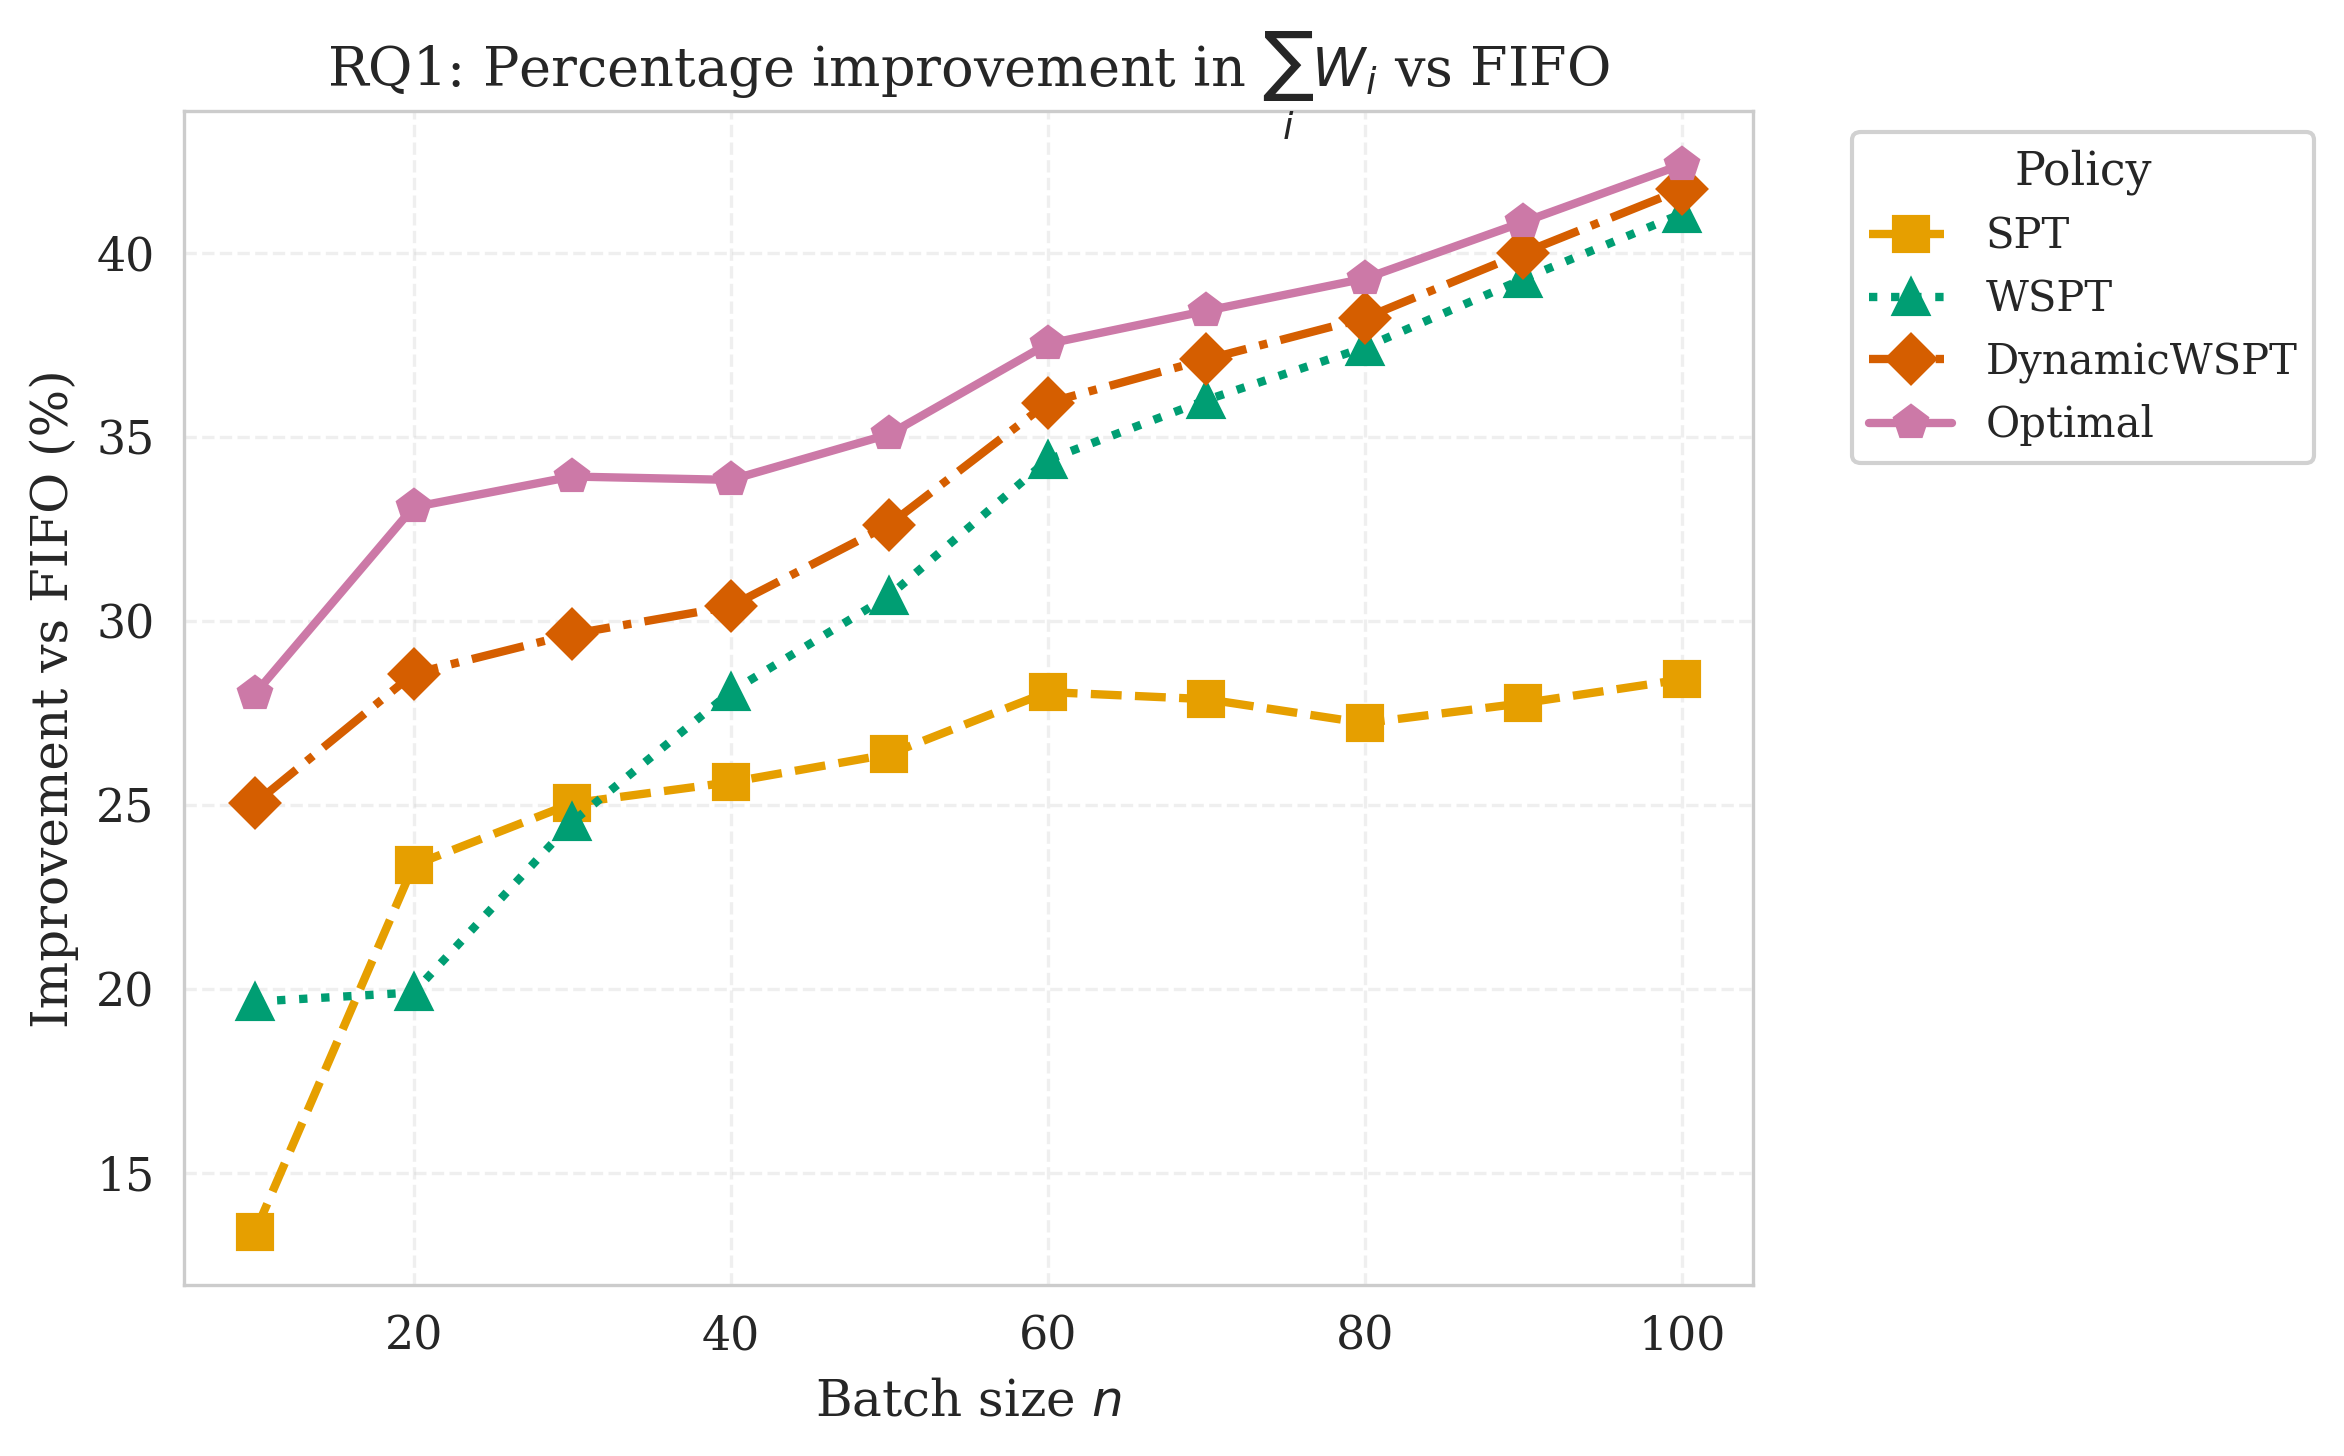
\includegraphics[width=0.9\linewidth]{rq1_improvement_vs_fifo_results_seeds20.png}
  \caption{Single activity: mean flow-time cost of SPT, WSPT, DynamicWSPT, and DP-optimal w.r.t. FIFO.}
  \label{fig:rq1_fifo}
\end{figure}

\paragraph{RQ2 (OR gateway: synchronization under heterogeneous bundles).}
\emph{Do valuation-driven policies reduce join delay in inclusive OR fragments where cases require different subsets of activities?}
We simulate an OR fragment with $m{=}3$ activities, each case requires each activity independently with probability $q{=}0.5$ and completes when all its required branches finish. We compare per-activity FIFO and SPT to \emph{SyncAware}, a bid-based policy that estimates the welfare gain from prioritizing case $i$:
$b_i=\int_{\tau_i^{v}}^{\tau_i^{H}} v_i(u)\,du$, where $\tau_i^{H}$ is predicted completion under FIFO and $\tau_i^{v}$ under prioritization. Bids are split across required activities so queues prioritize cases that most benefit from earlier synchronized completion.
SyncAware can be interpreted as a system-level extension of SPT. Instead of prioritizing cases by local processing times, it prioritizes them by their global marginal contribution to synchronized completion,
yielding a pressure-based rule conceptually analogous to Max-Pressure control
\citep{weikdd2019presslight}.

\begin{figure}[t]
  \centering
  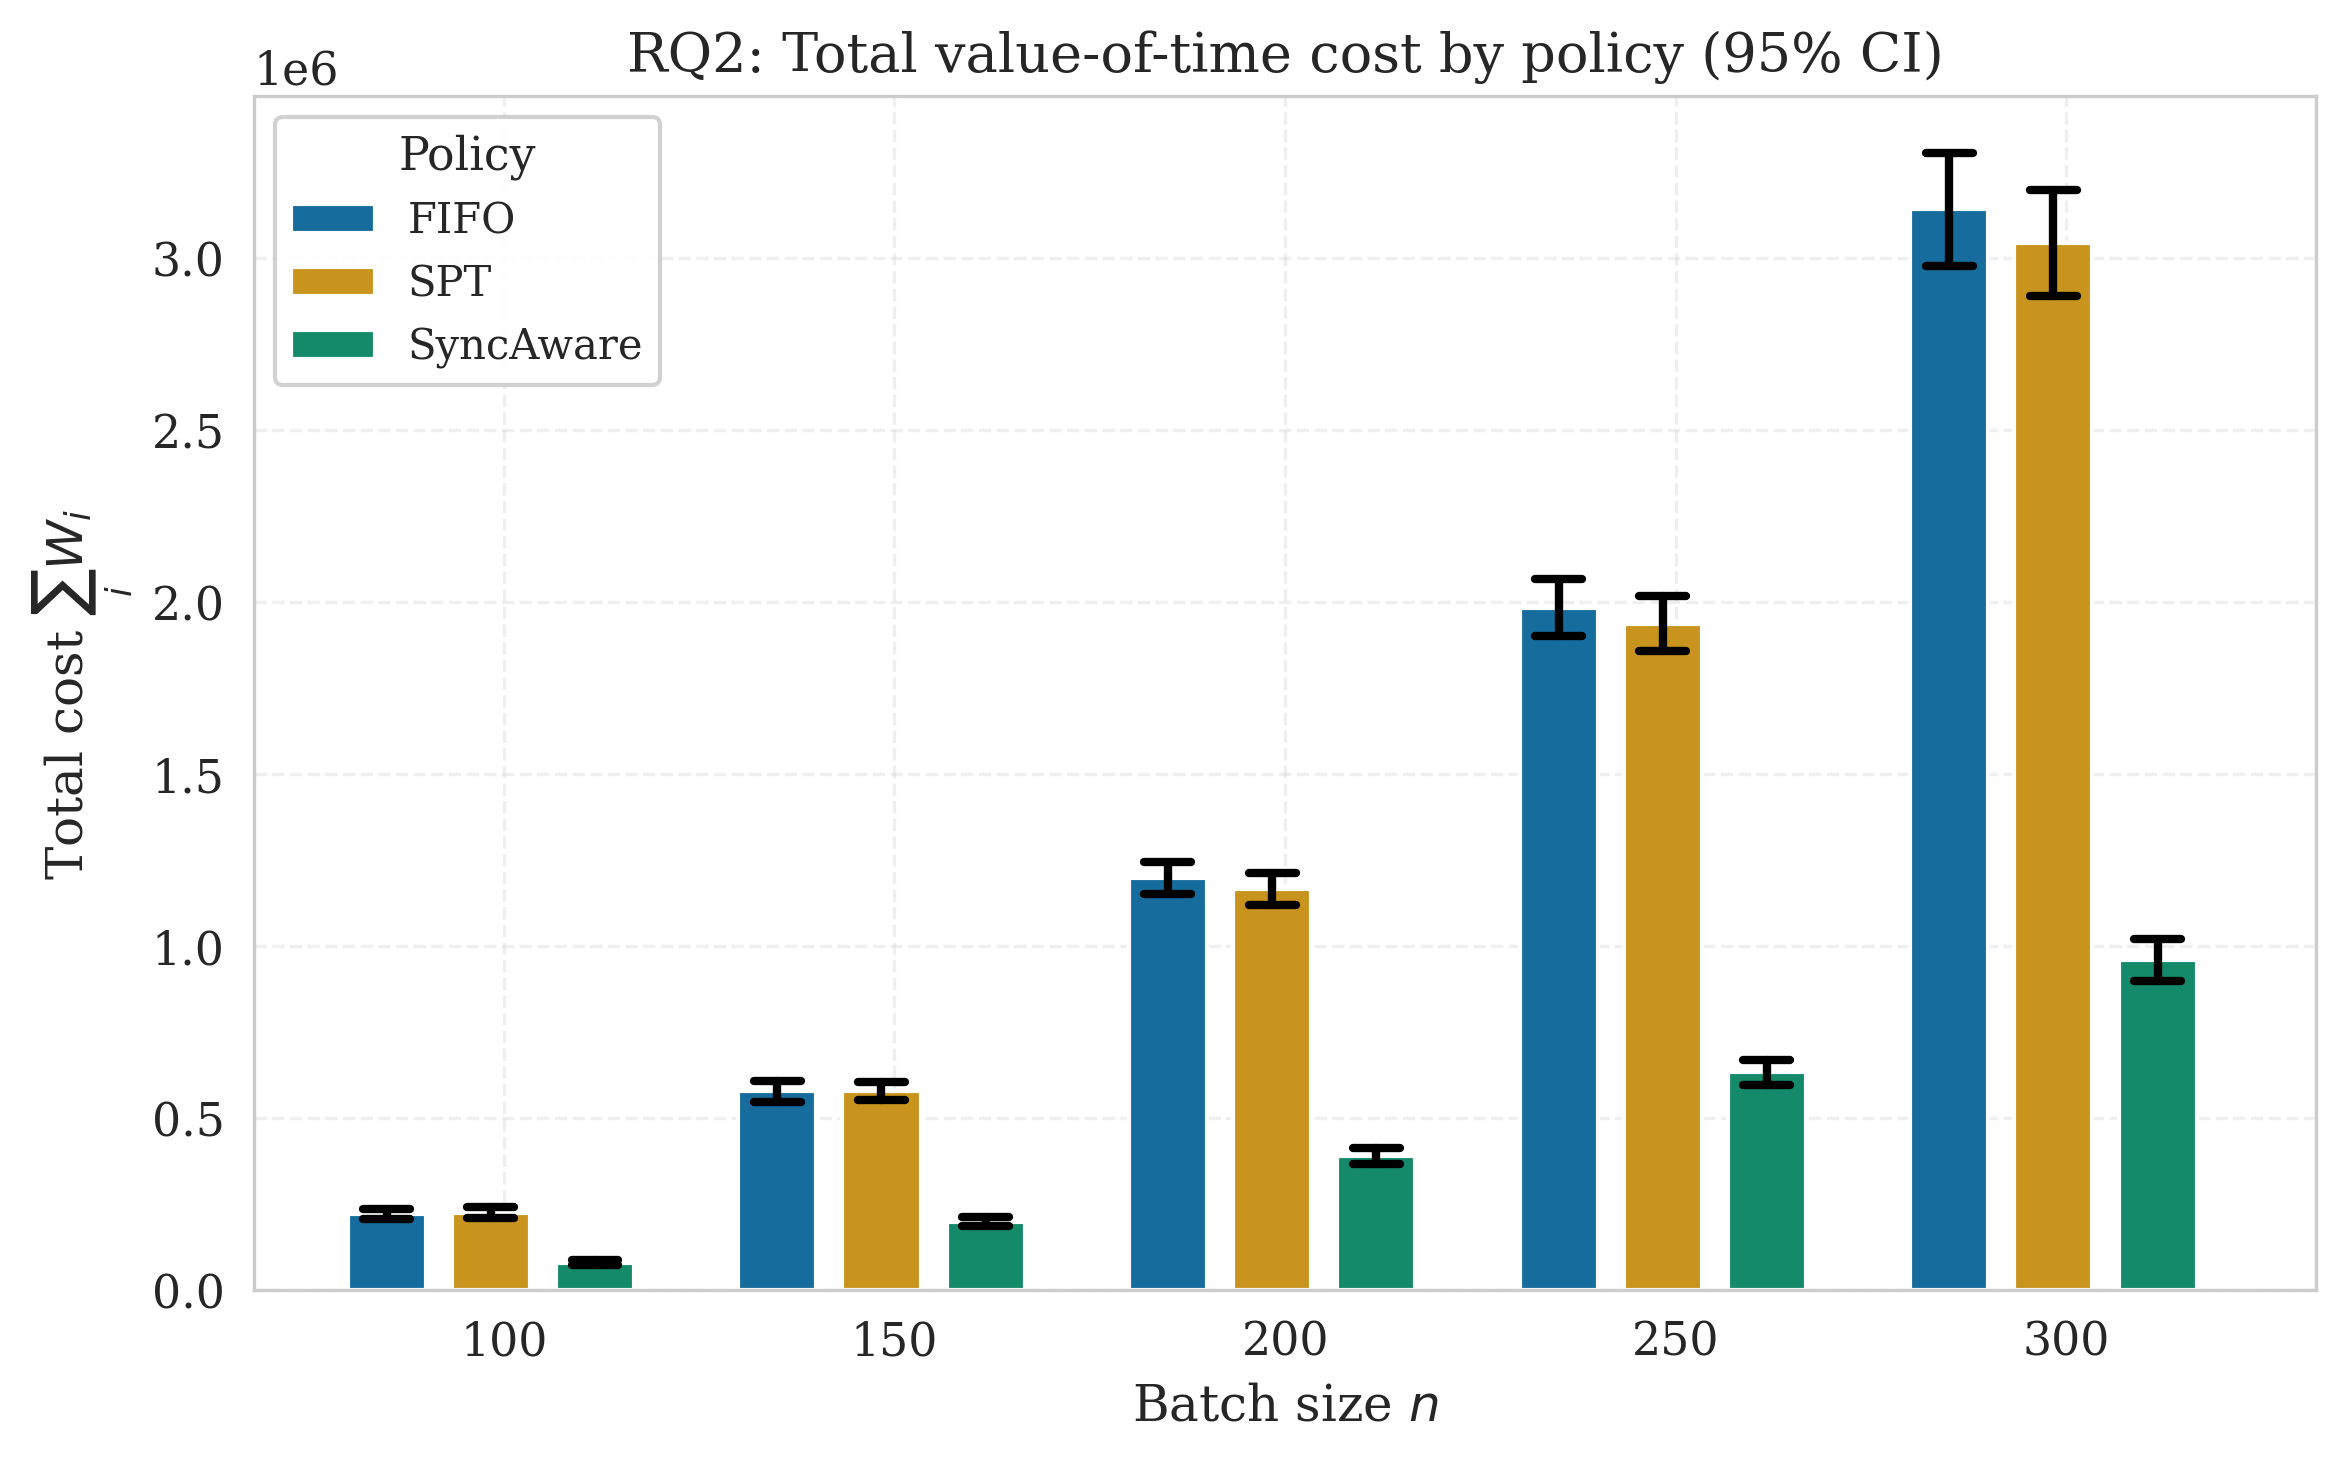
\includegraphics[width=0.9\linewidth]{rq2_total_cost_rq2_results_m3_q0.5_seeds20.png}
  \caption{OR gateway: mean total cost under FIFO, SPT, and SyncAware.}
  \label{fig:rq2}
\end{figure}

As shown in Figure~\ref{fig:rq2}, \emph{SyncAware} consistently improves welfare by internalizing cross-branch externalities that local heuristics ignore.



\paragraph{RQ3 (AND gateway: structural limits of per-activity rules).}
\emph{How much can synchronization-aware allocation help when all cases require all activities?}
We study an AND fragment with $m{=}5$ activities (each case requires all), constant valuations $V_i\sim U[0,100]$, and exponential processing times (activity $a\sim \mathrm{Exp}(a{+}1)$), varying $n\in\{200,300,400,500\}$. We compare FIFO, SPT, WSPT (per activity using $V_i/p_{i,a}$), and an \emph{AllocationHeuristic} that ranks cases by a critical-path ratio
$\pi(i)=V_i/\max_{a} p_{i,a}$ and allocates a selected case across required activities concurrently when capacity allows.
Figure~\ref{fig:rq3} shows that explicitly coordinating allocation across activities reduces synchronization-induced waiting relative to purely local dispatching.

\begin{figure}[t]
  \centering
  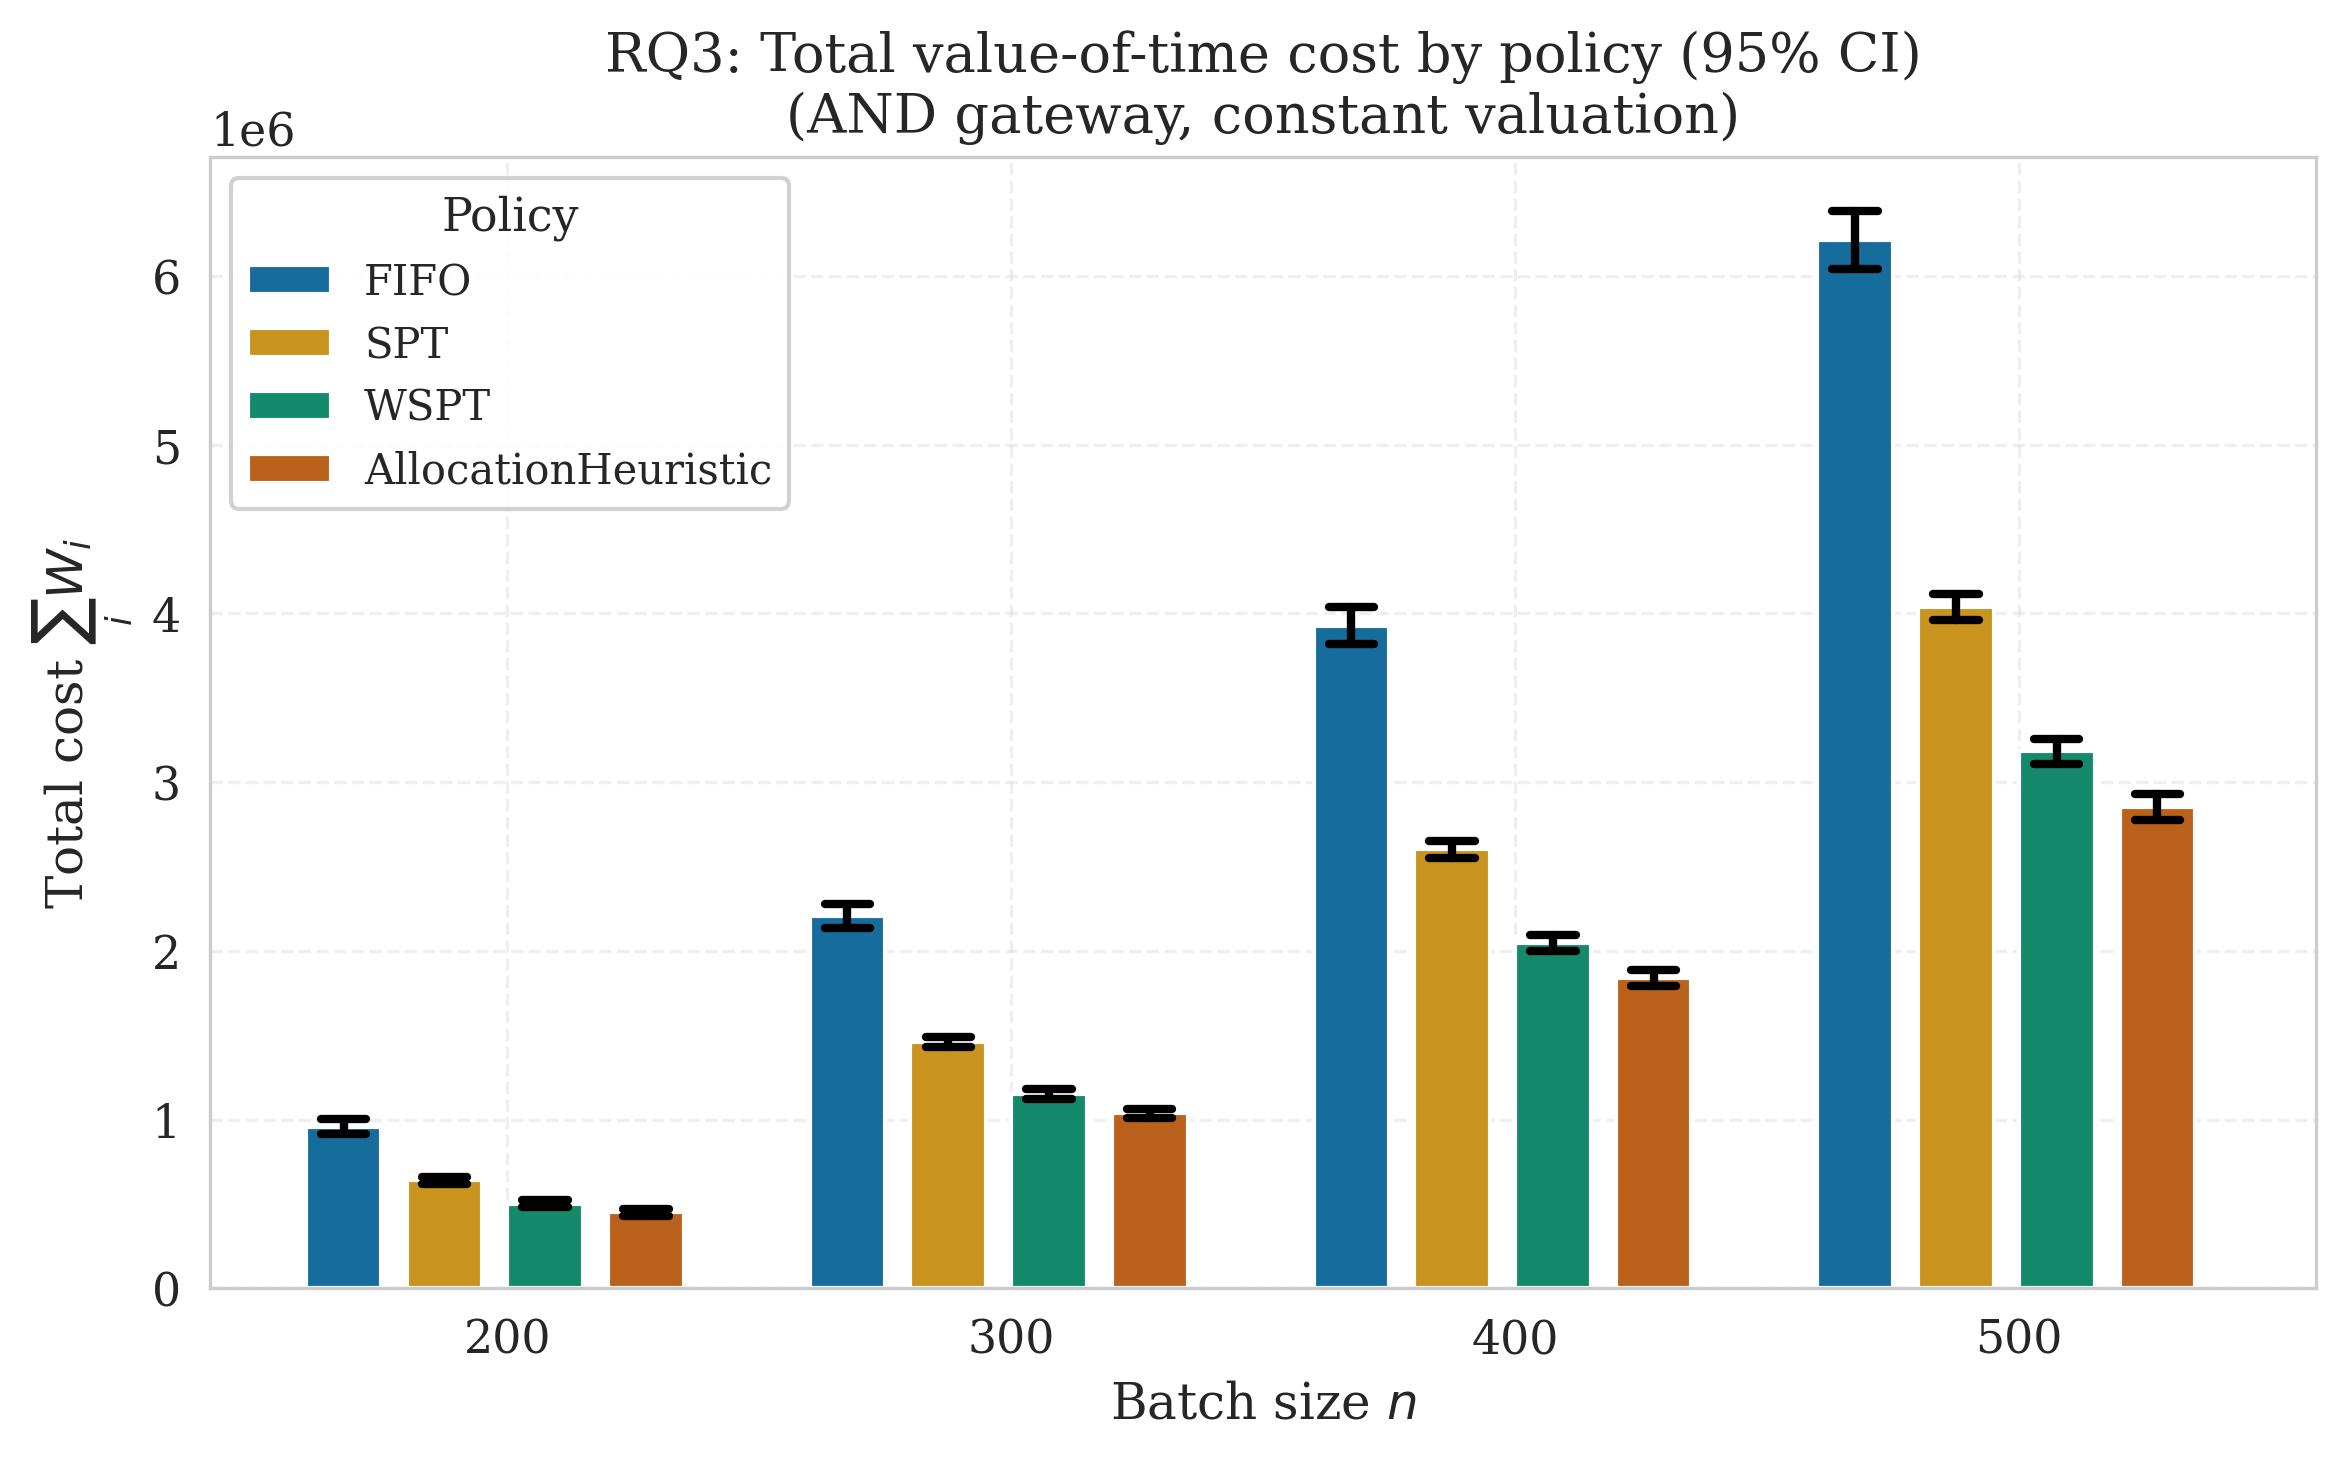
\includegraphics[width=0.9\linewidth]{rq3_total_cost_rq3_results_n200_300_400_500_seeds20.png}
  \caption{AND gateway: mean total cost under FIFO, SPT, WSPT, and AllocationHeuristic.}
  \label{fig:rq3}
\end{figure}

\paragraph{Takeaway.}
Across all settings, welfare losses arise from heterogeneity in delay sensitivity and, in routed fragments, from synchronization externalities. Valuation-driven policies use a value-of-time signal to align local prioritization with global completion dynamics, yielding robust improvements and narrowing the gap to optimal scheduling.




\section{Related work}
\label{sec:related}


% \ag{when describing related work, for each subsection conclude with a description of how our work differs from existing literature, either better or orthogonal}
\noindent\textbf{Workflow Gateways and Scheduling Structures.}
Workflow models describe processes as directed graphs in which
cases traverse activities and gateways \citep{dumas2018fundamentals}. From a
scheduling viewpoint, different gateways induce different structures.
An XOR-gateway corresponds to routing each case to exactly one branch,
an AND-gateway corresponds to an open shop where each case must visit
all branches \citep{lawler1993sequencing} and an OR-gateway allows each case
to require an arbitrary subset of branches, yielding a partial
concurrent open shop with synchronization at the join
\citep{senderovich2016conformance}. This OR structure strictly generalizes XOR
and AND and creates exponentially many case-types and feasible
sequences.
Where prior studies characterize the structural implications \citep{vanderaalst2003workflow,krishna2019checking}, 
they do not leverage these structures to design valuation-driven, incentive-compatible 
scheduling rules. Our work uses these gateway semantics as a foundation for defining 
strategic case preferences and deriving gateway-level dispatching mechanisms.

\noindent\textbf{Scheduling Theory for Open Shops and PCOS.} OR-gateways induce a partial concurrent open shop (PCOS), where each
case requires an arbitrary subset of activities and completes upon
synchronization at the join \citep{graham1979optimization}. Optimizing schedules in PCOS is NP-hard \citep{lawler1993sequencing}, and
standard heuristics such as FIFO, SPT, and priority rules can be
structurally misaligned with join synchronization\citep{gonzalez1976open}.

Existing open-shop and PCOS results primarily optimize processing-time
criteria and machine constraints, typically omitting synchronization-aware
delay externalities, online decision-making, and heterogeneous
case-specific delay costs \citep{graham1979optimization,grinshpoun2017pcos}.
As a result, they offer limited guidance for valuation-driven scheduling
in workflow nets with OR-routing. Our framework fills this gap by
combining PCOS structure with value-of-time functions and VCG-style
reasoning.



\noindent\textbf{Strategic Scheduling and VCG Mechanisms.} Strategic behavior in queues has been extensively studied in models
where each customer competes for a \emph{single} position in a
\emph{single} queue. VCG mechanisms
can implement welfare-maximizing priorities by charging delay
externalities \citep{lui1985bribery,hassin2003queue,nisan2007agt}.

This abstraction breaks down in workflow nets. A case may wait in
several queues simultaneously and must synchronize at a join, so its
utility depends on \emph{bundles} of positions across multiple
activities \citep{graham1979optimization}. Under OR-routing, a direct
VCG formulation would require reporting over an
exponential space of such bundles, rendering both preference elicitation
and winner determination computationally infeasible.

This places workflow scheduling exactly at the intersection of queueing
externalities and multi-parameter mechanism design. Most truthful scheduling results apply to \emph{single-parameter}
domains, where each job has a single private value and VCG mechanisms
remain tractable \citep{archer2001truthful,heydenreich2009games}. In contrast, \emph{multi-parameter} scheduling—where jobs value
combinations of machines or start times—is generally intractable due to
its combinatorial valuation space
\citep{dobzinski2008truthful,conitzer2006computational}. OR-routing in
business processes induces exactly this multi-dimensional structure:
each case values coordinated access to multiple activities
\citep{sandholm2002algorithm}.

This gap motivates a compact \emph{decision abstraction},  represented by a
low-dimensional signal that supports algorithmic reasoning.
As a result, it enables VCG-style externality pricing in synchronization-constrained
workflow settings that are not addressed by either classical queueing
mechanisms or existing multi-parameter scheduling models.
% \subsection{Learning Resource Allocation Policies}

% Recent work has explored learning resource allocation policies in business processes
% using reinforcement learning and simulation
% \citep{meneghello2024hybrid,meneghello2025proactive,middelhuis2025learning}. These approaches
% typically rely on sparse and domain-specific reward shaping, such as
% penalizing long cycle times or tardiness per case. Our value-of-time
% perspective suggests a more structured and dense reward signal:
% instantaneous value-of-time aggregated over cases currently in the
% system, which can drive RL agents to learn case-aware, welfare-oriented
% resource allocation.

\section{Conclusion}
\label{sec:conclusion}

% =====================================

We proposed a value-of-time based framework for strategic, case-aware scheduling
in business processes, built on three key ingredients:
(i) representing case preferences as temporal value-of-time functions,
(ii) interpreting these functions as compact, implicit valuations over bundles of
queue positions, enabling externality pricing and VCG-style reasoning at gateways,
and (iii) organizing XOR, AND, and OR routing into a taxonomy of six
scheduling regimes.
This taxonomy clarifies when classical heuristics are structurally aligned
with synchronization, when AND and OR routing fundamentally breaks local priority rules,
and how valuation heterogeneity can be exploited to improve welfare. We further showed that several
important special cases admit locally and globally optimal solutions.

Our framework opens several directions for future work. On the theoretical side,
a deeper characterization of tractable subclasses of partial concurrent open shops
with OR-routing, together with formal approximation and hardness results, remains open.
On the mechanism-design side, a full game-theoretic analysis of value-of-time reporting
and externality pricing in stochastic, networked BPM environments, where service times,
arrivals, and routing are subject to uncertainty is an important next step.
Lastly, extending the framework from individual process fragments to full process networks opens the door to learnable control systems that internalize delay externalities end to end.
% We proposed a value-of-time based framework for strategic case-aware
% scheduling in business processes, built on three main ingredients: (i) representing case
% preferences as temporal value-of-time functions, (ii) interpreting
% these functions as implicit valuations over bundles of queue positions
% to enable VCG-style reasoning at gateways, and (iii) organizing XOR,
% AND, and OR-routing into a unified taxonomy of seven
% scheduling cases. This taxonomy clarifies when FIFO and other heuristics suffices, when
% structural features of OR-routing demand more sophisticated policies,
% and how valuation heterogeneity can be exploited to improve welfare
% while remaining compatible with BPM models used in practice.

% We further showed that several important special cases admit explicit optimal solutions, including constant valuation for each case and fixed finite-type populations with fully general time-dependent valuation functions.


% Several directions remain open. On the theory side, a more detailed
% characterization of tractable subclasses of partial concurrent open
% shops with OR-routing is needed, along with formal approximation and
% hardness results. On the mechanism-design side, a full game-theoretic
% analysis of value-of-time reporting with VCG payments in stochastic,
% networked BPM environments is an important next step. 
% On the learning
% side, integrating valuation-based rewards with process mining,
% simulation, and RL at scale may yield practical, deployable
% case-aware scheduling policies for real-world service systems.

\smallskip
\noindent

% =========================
% BODY
% =========================
% \section{Introduction}
% ...

% =========================
% REFERENCES
% =========================
\bibliographystyle{named}
\bibliography{ijcai26} % <-- matches ijcai26.bib
\clearpage

\appendix
\newpage
\newpage
\section{Technical Appendix}
\subsection{Truthful reporting of value-of-time functions}
An \emph{allocation} $y\in\mathcal{X}$ specifies a feasible execution of the workflow fragment,
including the case-selection decisions at all activities over time.
Given an admissible policy $y\in\mathcal{X}$, case $i$ incurs
a waiting cost determined by the induced completion time:
\[
W_i(y;v_i)\ :=\ \int_{t}^{\tau_i(y)} v_i(u)\,du .
\]
Thus, any ``bundle valuation'' used by the mechanism is \emph{implicit}:
it corresponds to the negative of this cost under the completion time induced by the
bundle/policy.

\begin{lemma}[Truthfulness reporting]
\label{lem:truthful}
Each case $i$ reports a value-of-time function $\hat v_i(\cdot)$.
The planner selects an admissible allocation
\[
x \in \arg\min_{y \in \mathcal{X}} 
\sum_{k} W_k(y; \hat v_k),
\]

Payments are defined relative to a fixed baseline policy $\pi^{H}$ as
\begin{align*}
p_i(\hat v)
&:=
\sum_{j \neq i}
\Big(
W_j(\pi^{H}; \hat v_j)
-
W_j(x; \hat v_j)
\Big) \\[0.5em]
&=
\sum_{j \neq i}
\left(
\int_{t}^{\tau_j^{H}} \hat v_j(u)\,du
-
\int_{t}^{\tau_j(x)} \hat v_j(u)\,du
\right) \\[0.5em]
&=
\sum_{j \neq i}
\int_{\tau_j(x)}^{\tau_j^{H}}
\hat v_j(u)\,du .
\end{align*}


Then truthful reporting $\hat v_i = v_i$ is a dominant strategy within the reporting model for every
case $i$.
\end{lemma}

\begin{proof}
Fix the reports $\hat v_{-i}$ of all other cases.
The utility of case $i$ under its true value-of-time function $v_i$ is

\begin{align*}
u_i(\hat v_i, \hat v_{-i}; v_i)
&=
- W_i(x; v_i) - p_i(\hat v_i, \hat v_{-i}) \\[0.5em]
&=
- W_i(x; v_i)
-
\sum_{j \neq i}
\Big(
W_j(\pi^{H}; \hat v_j)
-
W_j(x; \hat v_j)
\Big) \\[0.5em]
&=
-
\Big(
W_i(x; v_i)
+
\sum_{j \neq i} W_j(x; \hat v_j)
\Big) +\\[0.25em]
&\hspace{2em}
+
\sum_{j \neq i} W_j(\pi^{H}; \hat v_j).
\end{align*}


The last term,
$\sum_{j \neq i} W_j(\pi^{H}; \hat v_j)$,
does not depend on $\hat v_i$.
Therefore, maximizing $u_i$ over all possible reports $\hat v_i$
is equivalent to minimizing
\[
W_i(x; v_i)
+
\sum_{j \neq i} W_j(x; \hat v_j)
\quad
\text{over } x.
\]

When case $i$ reports truthfully, $\hat v_i = v_i$,
the allocation rule selects
\[
x(v_i, \hat v_{-i})
\in
\arg\min_{x \in \mathcal{X}}
\Big(
W_i(x; v_i)
+
\sum_{j \neq i} W_j(x; \hat v_j)
\Big),
\]
which minimizes the above objective.
Hence, no deviation in the reported value-of-time function
can improve the utility of case $i$.
Truthful reporting is therefore a dominant strategy.
\end{proof}

This lemma establishes strategic truthfulness of the reporting
interface, independently of the computational tractability of
the induced allocation problem.


\begin{lemma}[Individual rationality via non-participation]\label{lem:IR-optout}
Extend the mechanism as follows: a case may \emph{not participate} by reporting
$\hat v_i(t)\equiv 0$, in which case it is scheduled last (tie-breaking rule) and
is charged $p_i=0$.
Then, for every true type $v_i(\cdot)$ and every reports $\hat v_{-i}$ of the other
cases, truthful reporting is individually rational:
\[
u_i(v_i,\hat v_{-i};v_i)\ \ge\ 0.
\]
\end{lemma}

\begin{proof}
Fix $\hat v_{-i}$. By Lemma~3 (dominant-strategy truthfulness),
truthful reporting maximizes $i$'s utility among all reports:
\[
u_i(v_i,\hat v_{-i};v_i)\ \ge\ u_i(\hat v_i,\hat v_{-i};v_i)
\quad \text{for all } \hat v_i.
\]
In particular, consider the \emph{non-participation} report $\hat v_i\equiv 0$.
By the mechanism definition, $p_i(0,\hat v_{-i})=0$, and since $\hat v_i\equiv 0$
corresponds to a delay-indifferent case, its utility under non-participation is
\[
u_i(0,\hat v_{-i};v_i)\ =\ -W_i(\text{scheduled last};v_i)\ -\ 0.
\]
Under the adopted outside-option convention (non-participation), the case is
treated as indifferent and normalized to utility $0$, i.e.,
$u_i(0,\hat v_{-i};v_i)=0$.
Therefore,
\[
u_i(v_i,\hat v_{-i};v_i)\ \ge\ u_i(0,\hat v_{-i};v_i)\ =\ 0,
\]
which proves individual rationality.
\end{proof}



\subsection{Proof of Lemma~\ref{lem:dyn-wspt}}
   \begin{proof}
Under $i\prec j$, $C_i=t+p_i$, $C_j=t+p_i+p_j$, hence
\[
J(i\prec j)=\int_{t}^{t+p_i} v_i(u)\,du+\int_{t}^{t+p_i+p_j} v_j(u)\,du.
\]
Under $j\prec i$, $C_j=t+p_j$, $C_i=t+p_j+p_i$, hence
\[
J(j\prec i)=\int_{t}^{t+p_j} v_j(u)\,du+\int_{t}^{t+p_j+p_i} v_i(u)\,du.
\]
Therefore
\[
\Delta:=J(i\prec j)-J(j\prec i)
=-\!\int_{t+p_i}^{t+p_j+p_i}\! v_i(u)\,du +
\]
\[
+\!\int_{t+p_j}^{t+p_i+p_j}\! v_j(u)\,du .
\]
Thus $i\prec j$ is weakly better (i.e., $\Delta\le0$) iff
\[
\int_{t+p_j}^{t+p_i+p_j}\! v_j(u)\,du
\ \le\
\int_{t+p_i}^{t+p_j+p_i}\! v_i(u)\,du .
\]
Divide both sides by the \emph{common} factor $p_ip_j$ (rather than by different window lengths) to obtain
\[
\frac{1}{p_j}\,\frac{1}{p_i}\!\int_{t+p_j}^{t+p_i+p_j}\! v_j(u)\,du
\ \le\
\frac{1}{p_i}\,\frac{1}{p_j}\!\int_{t+p_i}^{t+p_j+p_i}\! v_i(u)\,du,
\]
i.e.,
\[
\frac{\tilde v_j(t, p_i)}{p_j}\ \le\ \frac{\tilde v_i(t, p_j)}{p_i}.
\]
If $v_i(u)\equiv c_i$ is constant, then $\tilde v_j(t,p_i)=c_j$ and $\tilde v_i(t,p_j)=c_i$, so the condition becomes
$c_j/p_j \le c_i/p_i$, which is WSPT rule. 
If $c_i$ is equal for all cases, this is SPT. 
\end{proof}



\subsection{Proof of Theorem~\ref{thm:ncase-local} and Algorithm~\ref{alg:alg1}}
\begin{proof}
The proof extends Lemma~\ref{lem:dyn-wspt} to a full queue.
For any $k$, consider the local interval
$[s_k,\,s_k+p_{k}+p_{{k+1}}]$ that covers the processing of the two
adjacent cases $k$ and ${k+1}$.
Only these two cases contribute differently to $J$ within this interval. Earlier parts are identical and later parts are unaffected.

By Lemma~\ref{lem:dyn-wspt},
\[
\Delta J(({k+1}\prec k))-\Delta J((k\prec {k+1}))
\]
\\
\[
=\int_{s_k+p_{k}}^{s_k+p_{k}+p_{{k+1}}}\! v_{k}(u)\,du
-\int_{s_k+p_{{k+1}}}^{s_k+p_{k}+p_{{k+1}}}\! v_{{k+1}}(u)\,du.
\]
Condition \eqref{eq:pair-condition-local} makes this difference nonnegative,
hence swapping $k$ and ${k+1}$ cannot reduce $J$ on that interval.
Therefore, no \emph{adjacent} swap can improve $J$, i.e., $\sigma$ is locally optimal.
\end{proof}




\begin{algorithm}[t!]
\caption{Dynamic Local Reordering of Cases}
\label{alg:alg1}
\begin{algorithmic}
\Require Set of ready cases $\mathcal{I}$, processing times $\{p_i\}$, value functions $\{v_i(\cdot)\}$, current time $t$
\State Initialize any order. Set $s_1\gets t$
\Repeat
  \State $\textit{changed}\gets \textbf{false}$
  \For{$k=1$ \textbf{to} $n-1$}
    \State Compute for the adjacent pair $(k,{k+1})$:
      \[
      A = \int_{s_k+p_{{k+1}}}^{s_k+p_{k}+p_{{k+1}}} v_{{k+1}}(u)\,du ,
      \]
      \[
      B = \int_{s_k+p_{k}}^{s_k+p_{k}+p_{{k+1}}} v_{k}(u)\,du.
      \]
    \If{$A > B$}
        \State swap case $k$ and ${k+1}$ in $\sigma$;
        \State $\textit{changed}\gets \textbf{true}$.
    \EndIf
    \State $s_{k+1}\gets s_k+p_{k}$
  \EndFor
\Until{$\textit{changed}=\textbf{false}$}
\State \Return $\sigma$ \quad (adjacent-exchange stable, locally optimal)
\end{algorithmic}
\end{algorithm}


\begin{remark}[Complexity and guarantee]
In general, pairwise-exchange stability \emph{does not} imply global optimality. The returned order is \emph{locally optimal} and dominants over FIFO.
Each swap strictly reduces the number of inversions, hence the procedure terminates after at most $\binom{n}{2}$ swaps, i.e., in $O(n^2)$ local exchanges.
The algorithm converges to a locally optimal order in $O(n^2)$ local exchanges.
\end{remark}



\subsection{Max-Plus}

\begin{proof}
Under $\pi^{\mathrm{inv}}$ (order $i\prec_1 j$ and $j\prec_2 i$),
\[
C_i^{\mathrm{inv}} = p_{i1}\;\oplus\;(p_{j2}\otimes p_{i2}),\qquad
C_j^{\mathrm{inv}} = (p_{i1}\otimes p_{j1})\;\oplus\;p_{j2}.
\]
Under $\pi^{i\prec j}$ (order $i$ then $j$ on both),
\[
C_i^{i\prec j} = p_{i1}\oplus p_{i2},\qquad
C_j^{i\prec j} = (p_{i1}\otimes p_{j1})\oplus (p_{i2}\otimes p_{j2}).
\]
Define 
$\Delta_i:=C_i^{\mathrm{inv}}-C_i^{i\prec j}\ge 0 , \
\Delta_j:=C_j^{i\prec j}-C_j^{\mathrm{inv}}\ge 0,$

where non-negativity follows from monotonicity of $\oplus$ and $\otimes$.
Therefore,
\[
W(\pi^{\mathrm{inv}})-W(\pi^{i\prec j})
=V_i\Delta_i - V_j\Delta_j.
\]
If $V_i\Delta_i\ge V_j\Delta_j$ then $W(\pi^{i\prec j})\le W(\pi^{\mathrm{inv}})$,
so $\pi^{i\prec j}$ dominates the inversion.

Otherwise $V_i\Delta_i< V_j\Delta_j$. By symmetry, comparing $\pi^{\mathrm{inv}}$
to $\pi^{j\prec i}$ yields
$W(\pi^{\mathrm{inv}})-W(\pi^{j\prec i})=V_j\widetilde{\Delta}_j-V_i\widetilde{\Delta}_i$
with $\widetilde{\Delta}_j,\widetilde{\Delta}_i\ge 0$, and in this complementary
regime the inequality implies $W(\pi^{j\prec i})\le W(\pi^{\mathrm{inv}})$.
Hence at least one of the two consistent permutations is no worse than the
inversion, proving the claim.
\end{proof}

\begin{theorem}[Permutation-consistent dominance for AND with constant valuations]\label{thm:and-perm-m}
Consider an AND-gateway with $m$ parallel activities $a\in[m]$ and $n$ cases
$i\in[n]$, each requiring all activities. Assume non-preemptive service with
deterministic processing times $p_{i,a}$ and constant valuations $V_i>0$.
Let each activity $a$ process cases according to a (possibly different) local
order, inducing per-activity completion times $C_{i,a}$ and join times
$C_i=\bigoplus_{a\in[m]} C_{i,a}$. The welfare objective is
$W=\sum_{i=1}^n V_i C_i$.
Then for any order profile $\pi=(\pi_1,\ldots,\pi_m)$ there exists a
permutation-consistent profile $\pi'=(\sigma,\ldots,\sigma)$ such that
$W(\pi')\le W(\pi)$. Equivalently, there always exists an optimal schedule whose
per-activity orders are identical.
\end{theorem}

\begin{proof}[Proof of Theorem~\ref{thm:and-perm-m}]
Fix any schedule profile $\pi=(\pi_1,\ldots,\pi_m)$. We show how to transform it
into a permutation-consistent profile without increasing welfare.

Fix an anchor activity, say $a_1$, with order $\pi_1$. For each other activity
$a_r \in \{2,\ldots,m\}$, we will modify $\pi_r$ and  so that it  matches $\pi_1$.
Consider a step in which $\pi_r$ disagrees with $\pi_1$. Then there exists an
inverted adjacent pair of cases $(i,j)$ such that $i\prec_{1} j$ but $j\prec_{r} i$.

Freeze all cases other than $i,j$, and freeze all activities other than the pair
$(a_1,a_r)$. Under this restriction, the join times of $i$ and $j$ still have the
max-plus form
\[
C_i = C_{i1}\oplus C_{ir}\oplus H_i,\qquad
C_j = C_{j1}\oplus C_{jr}\oplus H_j,
\]
where $H_i:=\bigoplus_{a\in[m]\setminus\{1,r\}} C_{i,a}$ and similarly for $H_j$
are constants with respect to the relative order of $(i,j)$ on $a_r$.


Now view $(a_1,a_r)$ as a two-activity AND subproblem for the two cases $(i,j)$,
with constant valuations $(V_i,V_j)$ and (fixed) offsets captured by $(H_i,H_j)$.
The current relative order constitutes an inversion between the two activities.
By Lemma~\ref{lem:inv-dominated}, this inverted profile is weakly dominated by at
least one of the two permutation-consistent relative orders for $(i,j)$ (either
$i\prec j$ on both $a_1,a_r$ or $j\prec i$ on both), hence we can replace the
inversion by a consistent relative order without increasing the welfare
contribution of $i$ and $j$.

Implement this replacement by performing adjacent swaps on activity $a_r$ until
the relative order of $i$ and $j$ matches that of $a_1$. Since each swap only
reorders two adjacent cases on $a_r$, it affects only their completion times on
$a_r$. All other completion times $C_{k,a}$ ($k\notin\{i,j\}$ or $a\neq r$) remain
unchanged. Therefore, the total welfare does not increase in this step.

Repeat the above procedure until no inversions remain between $\pi_r$ and $\pi_1$,
i.e., until $\pi_r=\pi_1$. This terminates because each swap strictly decreases
the inversion count between $\pi_r$ and $\pi_1$, which is finite.
Applying this independently for all $r=2,\ldots,m$ yields a permutation-consistent
profile $\pi'=(\sigma,\ldots,\sigma)$ with $\sigma=\pi_1$ and $W(\pi')\le W(\pi)$.
Hence, an optimal permutation-consistent schedule exists.
\end{proof}





\end{document}
